\documentclass[10pt,a4paper]{article}
\usepackage[utf8]{inputenc}
\usepackage[english,russian]{babel}
\usepackage{cmap}
\usepackage[OT1]{fontenc}
\usepackage{amsmath}
\usepackage{amsfonts}
\usepackage{amssymb}
\usepackage{graphicx}
\usepackage{float}
\usepackage{wrapfig}
\usepackage{caption}
\DeclareCaptionLabelSeparator{dot}{. }
\captionsetup{justification=centering,labelsep=dot}
\graphicspath{{pictures/}}
\DeclareGraphicsExtensions{.pdf,.png,.jpg,.eps}
\begin{document}

\part{Основы}



\textbf{8 Локализация мобильного робота: методы Монте-Карло и построения сеток}\\

\textbf{8.1	Введение}\\

В этой главе описаны два алгоритма локализации, способных решать проблему глобальной локализации. Обсуждаемые здесь алгоритмы имеют ряд отличий от одномодальных гауссовых методов, обсуждаемых в предыдущей главе. \\

•	Они способны обрабатывать «сырые» показания датчиков. Нет необходимости извлекать признаки из данных показаний датчиков, что напрямую обеспечивает возможность обрабатывать отрицательную информацию. \\

•	Они непараметрические. В частности, они не привязаны к одномодальному распределению, как это было в случае с алгоритмом локализации EKF.\\

•	Они способны решать проблему глобальной навигации, а в некоторых реализациях – и похищенного робота. Алгоритм EKF на такое неспособен, хотя MHT (отслеживание нескольких гипотез) возможно модифицировать для решения задачи глобальной локализации.\\

Представленные методы показали великолепные результаты в ряде робототехнических систем, действующих в реальных условиях. 

Первый метод называется \textit{локализация по сетке}. В нем для отображения апостериорной оценки применен фильтр на основе гистограмм. С применением локализации по сетке связан ряд ограничений: при использовании мелкого разбиения сетки  вычислительные затраты, требующиеся для работы наивного алгоритма, неприемлемо велики. Для крупной сетки дополнительная потеря информации в результате дискретизации негативно влияет на фильтр и, если её корректно не обрабатывать, может даже нарушить его работу. 

\begin{table}[H]
\begin{center}
\begin{tabular}{|l|}
\hline
{}\\
1: \textbf{Algorithm Grid\_localization}$(\{p_{k,t-1}\},u_t,z_t,m):$ \\
2:\hspace{3mm}$\textit{for all k do}$\\
3:\hspace{7mm}$\bar{p}_{k,t}=\sum_i p_{i,t-1}\text{\textbf{motion\_model}}(\text{mean}(\text{x}_k),u_t,\text{mean}(\text{x}_i))$\\
4:\hspace{7mm}$p_{k,t}=\eta\,\bar{p}_{k,t}\text{\textbf{measurement\_model}}(z_t,\text{mean}(\text{x}_k),m)$\\
5:\hspace{3mm}$\textit{endfor}$\\
6:\hspace{3mm}$\textit{return}\,\{p_{k,t}\}$\\
{}\\
\hline
\end{tabular}
\caption{(Таблица 8.1 Локализация по сетке, вариант дискретного байесовского фильтра. Функция \textbf{motion\_model} реализует одну из моделей движения, а \textbf{measurement\_model}  - модель измерения. Функция “mean” возвращает центр масс ячейки сети $\text{x}_k$.)}
	\end{center}
\end{table}

Второй метод - это локализация методом Монте-Карло (Monte Carlo localization -MCL), наверное, самый популярный алгоритм локализации на сегодняшний день. В нем для получения апостериорных оценок положения робота используются многочастичные фильтры. Мы обсудим ряд недостатков MCL, а также представим варианты использования для задачи похищенного робота и динамических окружающих сред.
\\

\textbf{8.2	Локализация по сетке}\\

\textbf{8.2.1	Общий алгоритм}\\

В алгоритме \textit{локализации по сетке} апостериорное распределение аппроксимируется с использованием \textit{фильтра на основе гистограмм} в декомпозиции пространства положений в виде сетки. Дискретный байесовский фильтр уже был подробно объяснён в Главе 4.1 и приведен в Таблице 4.1. Апостериорное распределение хранится в виде набора значений вероятности \\

(8.1)
$$bel(x_t)=\{p_{k,t}\}$$

где каждая вероятность $p_{k,t}$ определена для ячейки сетки $\text{x}_k$. Набор всех ячеек сетки образует разбиение пространства всех возможных положений:\\

(8.2)
$$\text{domain}(X_t)=\text{x}_{1,t}\cup\text{x}_{2,t}\cup...\text{x}_{K,t}$$

В самой простой версии локализации по сетке разбиение пространства всех положений инвариантно по времени, и все ячейки одинакового размера. Для многих помещений популярно разбиение сеткой с ячейкой 15 см по осям $x$- и $y$, и 5 градусов для измерения поворота. Более мелкое представление даёт лучшие результаты, но ценой возросшей вычислительной нагрузки.

Локализация по сетке, по большей части, идентична базовому алгоритму фильтра на основе гистограмм, из которого она и произошла. В Таблице 8.1 приводится псевдокод для самой общей реализации. На вход необходимо подать дискретные значения вероятности $\{p_{t-1,k}\}$, а также самые последние измерения, действия управления и карту. Во внутреннем цикле выполняется перебор всех ячеек сетки. В строке 3 выполняется обновление модели движения, а в строке 4 –обновление измерения. Итоговые вероятности нормализуются с помощью нормализующего коэффициента $\eta$ в строке 4. Функции \textbf{motion\_model} и \textbf{measurement\_model} могут быть реализованы с помощью любой модели движения из Главы 5 и модели измерений из Главы 6, соответственно. В алгоритме в Таблице 8.1 допускается, что каждая ячейка имеет одинаковый размер.

На Рис. 8.1 показан пример локализации по сетке для случая одномерного коридора. Эта схема аналогична базовому байесовскому фильтру, за исключением дискретного способа реализации. Как и прежде, робот начинает в ситуации глобальной неопределённости, выраженной равномерной гистограммой. По мере сбора данных в соответствующих ячейках сетки возрастают значения вероятности. Пример явно иллюстрирует возможность представления мультимодальных распределений с помощью локализации по сетке. \\

\textbf{8.2.2	Разрешение сетки}\\

Ключевым параметром для алгоритмов локализации по сетке является разрешение сетки. На первый взгляд, это может показаться малозначительной деталью. Но подходящий тип модели датчика, вычислительные мощности, требующиеся для вычисления оценки и тип ожидаемого результата - все они зависят от разрешения сетки.

В конечном счёте, есть два типа отображений, каждый из которых успешно проявил себя в практических робототехнических системах.

ТОПОЛОГИЧЕСКОЕ ОТОБРАЖЕНИЕ

Общепринятым подходом является определение сетки в \textit{топологическом виде}.  Результирующие сетки обычно очень грубы, а их разрешение зависит от структуры окружающей среды. Топологические разбиения разбивают пространство всех положений на области, соответствующие \textit{важным местам} в окружающей среде. Такие места могут определяться по наличию (или отсутствию) определённых ориентиров, например, дверей и окон. В средах с коридорами такие места могут соответствовать пересечениям, разветвлениям, тупикам и так далее. Топологические отображения обычно довольно грубы, их разбиение среды зависит от структуры среды. На Рис. 8.5 показано такое разбиение для случая одномерного коридора. 

\begin{figure}[H]
	\center{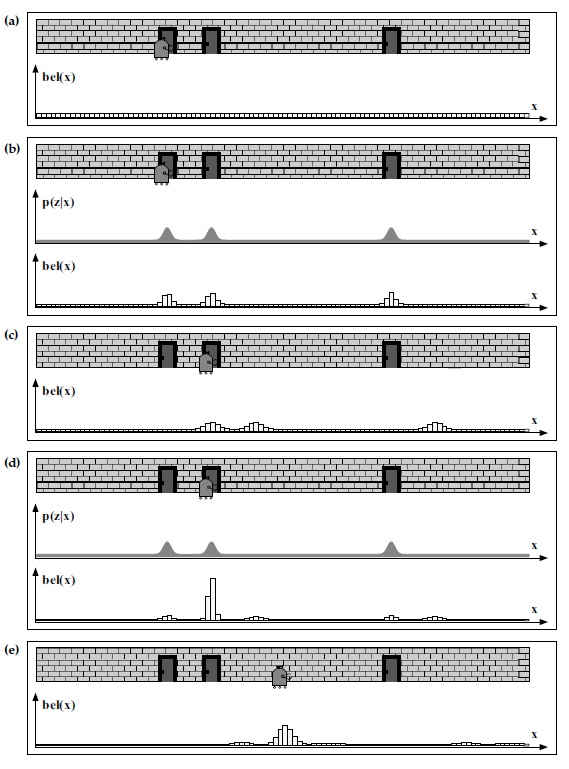
\includegraphics[width=1\linewidth]{81orig}}
	\caption{ (  Рис. 8.1 Сеточная локализация, на основе мелкого метрического разбиения. На каждой схеме показана позиция робота в коридоре согласно его оценке $bel(x_t)$ по сетке, отображённая в виде гистограммы .)}
	\label{fig:81orig}
\end{figure}

\begin{figure}[H]
	\center{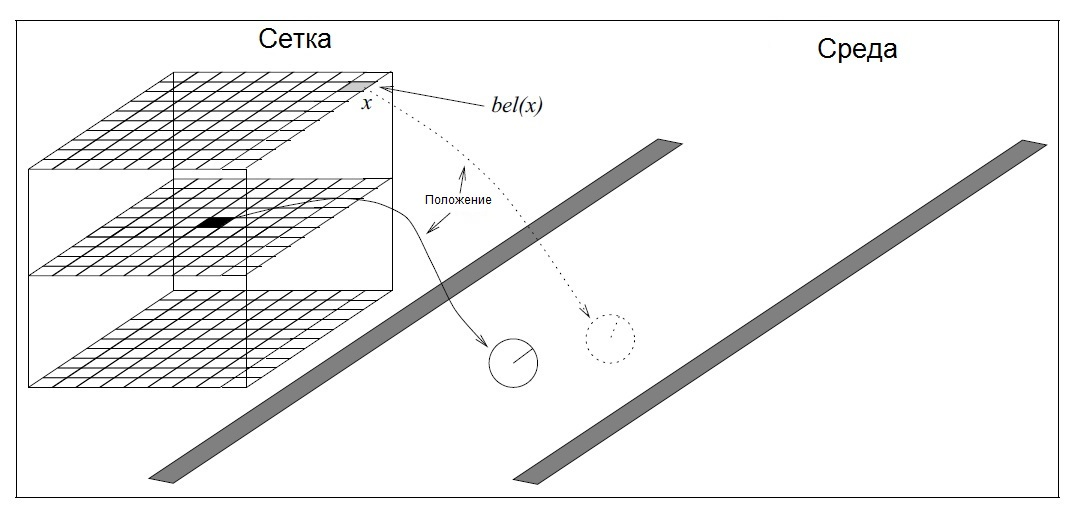
\includegraphics[width=1\linewidth]{82orig}}
	\caption{ (  Рис. 8.2 Сетка с фиксированным разрешением по переменным положения робота $x$,  $y$ и $\theta$. Каждая ячейка представляет собой положение робота в окружающей среде. Различные ориентации по углу направления соответствуют различным плоскостям сетки (показано только три ориентации).)}
	\label{fig:82orig}
\end{figure}

МЕТРИЧЕСКОЕ 
ПРЕДСТАВЛЕНИЕ

Значительно более мелкое разбиение обычно получается в \textit{метрических представлениях}, где пространство состояний разбивается на ячейки одинакового размера. Разрешение таких разбиений обычно гораздо более высокое, по сравнению с топологическими сетями. Например, в некоторых примерах Главы 7 используются разбиения сетки с размером ячейки 15 см или менее, в силу этого они более точны, но ценой возросшей вычислительной сложности. На Рис. 8.2 показана такая сеть с фиксированным разбиением. Мелкое разбиение, наподобие показанного, обычно используется в метрическом представлении пространства. 

При реализации локализации по сетке для грубых разбиений важно компенсировать разбиение разрешением моделей датчика и движения. В частности, для датчиков с высоким разрешением, наподобие лазерного датчика расстояния, значение модели измерения $p(z_t|x_t)$ может сильно варьироваться внутри каждой ячейки сетки $\text{x}_{k,t}$. В таком случае простая оценка с помощью центра масс обычно даёт плохие результаты. Аналогично, прогнозирование движения робота на основе данных о центре масс ячейки тоже может дать плохие результаты. Если движение обновляется с интервалами 1 сек для робота, который двигается со скоростью 10 см/сек, и разрешением сетки 1 метр, наивная реализация никогда не даст перехода состояния! Это происходит потому, что любое местонахождение, удалённое на 10 см от центра масс ячейки все ещё попадает внутрь одной и той же ячейки сетки. 

\begin{figure}[H]
	\center{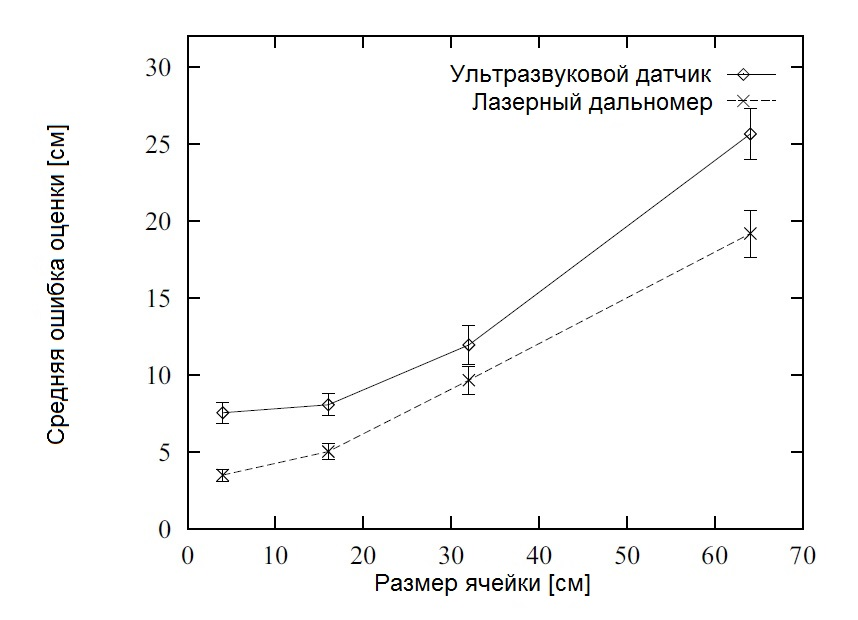
\includegraphics[width=1\linewidth]{83orig}}
	\caption{ (  Рис. 8.3 Средняя ошибка локализации ультразвуковых и лазерных датчиков расстояния как функция размера ячейки сети.)}
	\label{fig:83orig}
\end{figure}

Обычным способом компенсации этого эффекта является модификация как модели измерения, так и модели движения путём увеличения параметра зашумления. Например, дисперсия гауссовой модели основного конуса измерений датчика расстояния может быть увеличена на половину диаметра ячейки сети. Таким образом, новая модель станет значительно более гладкой, а ее интерпретация – менее подвержена зависимости от точного местоположения предполагаемой точки относительно истинного местоположения робота. С другой стороны, такая модифицированная модель измерений уменьшает количество информации, извлекаемой из измерений датчика.

Аналогично, и модель движения может выполнять прогнозирование случайного перехода на соседнюю ячейку с вероятностью, пропорциональной длине дуги движения, делённой на диаметр ячейки. Результатом работы такой огрублённой модели движения является возможность робота передвигаться от одной ячейки к другой, даже если его перемещение между последовательными обновлениями  относительно размера ячейки сети достаточно мало. Однако, результирующие апостериорные распределения неверны в том, что неоправданно высокая вероятность будет назначена гипотезе, в которой робот переходит в другую ячейку при каждом обновлении движения, а, значит, перемещается гораздо быстрее, чем было указано сигналами управления. 

\begin{figure}[H]
	\center{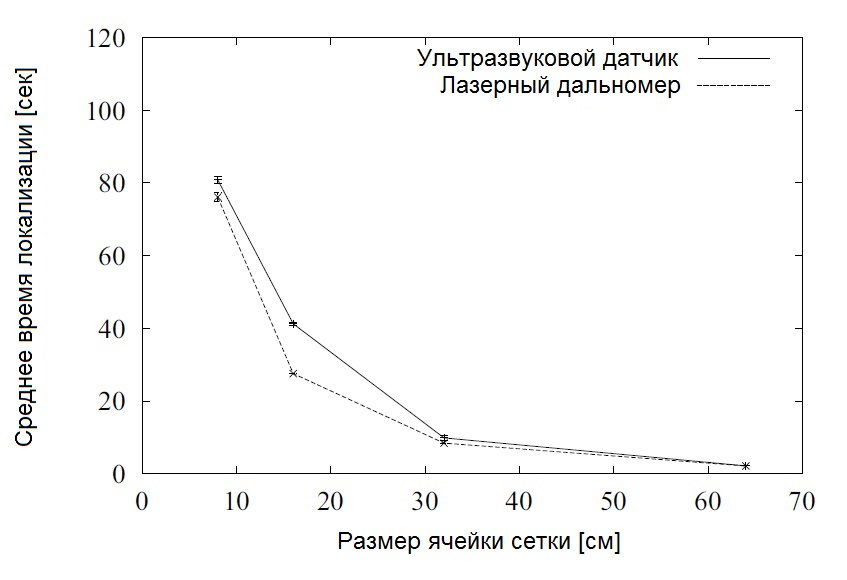
\includegraphics[width=1\linewidth]{84orig}}
	\caption{ ( Рис. 8.4 Средние затраты процессорного времени, необходимые для глобальной локализации с помощью ультразвукового и лазерного датчика расстояния как функция разрешения сети.)}
	\label{fig:84orig}
\end{figure}

На Рис. 8.3 и 8.4 показаны графики представления локализации по сетке в виде функции разрешения для разных датчиков расстояния. Как и ожидалось, ошибка локализации возрастает по мере уменьшения разрешения. Общее время, необходимое для локализации робота уменьшается по мере увеличения ячеек сети, как показано на Рис. 8.4.\\

\textbf{8.2.3	Вычислительные соображения}\\

При использовании сетки с мелкой ячейкой, наподобие описанных в примере в предыдущем разделе метрических сеток, общий алгоритм не может быть выполнен в реальном времени, поскольку ошибки возникают и при обновлении движения, и при обновлении измерения. Обновление движения требует выполнения свёртки, которая для трёхмерной сети является операцией в шести измерениях. Обновление измерения является операцией в трёх измерениях, но вычисление правдоподобия полного прохода сканирования весьма вычислительно затратно.

ПРЕДВАРИТЕЛЬНОЕ КЭШИРОВАНИЕ МОДЕЛИ

Существует ряд методов уменьшения вычислительной сложности локализации по сетке.
\textit{Предварительное кэширование модели} основано на том, что определённые модели измерений очень затратно вычислять. Например, вычисление модели измерения может потребовать бросания лучей, которые возможно предварительно вычислить для любой фиксированной карты. Как было указано в подразделе 6.3.4, общепринятой стратегией является вычисление для каждой ячейки основных статистик, влияющих на обновление измерения. В частности, при использовании модели на основе лучей принято кэшировать верное расстояние до каждой ячейки.  Далее, модель измерения может быть вычислена для набора возможных значений расстояния с мелким разбиением. Вычисление модели измерения сводится к операции просмотра двух таблиц, что значительно быстрее. 

\begin{figure}[H]
	\center{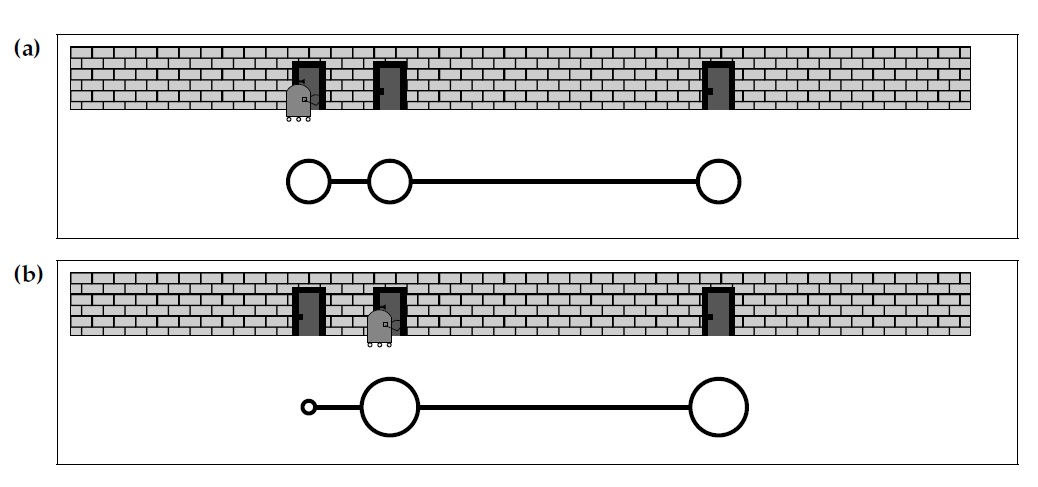
\includegraphics[width=1\linewidth]{85orig}}
	\caption{ ( Рис. 8.5 Применение грубого топологического разбиения для локализации мобильного робота. Каждому состоянию соответствует конкретное место в среде (в данном случае, около двери). Гипотеза робота $bel(x_t)$ о нахождении в конкретном состоянии отображена в виде размера кругов. (a) Начальная оценка равномерна по всем положениям (b) Показана оценка после одного перехода состояния и обнаружения двери. В этой точке маловероятно, что робот все ещё находится в крайней левой позиции. )}
	\label{fig:85orig}
\end{figure}

ПОДВЫБОРКА ЗНАЧЕНИЙ ДАТЧИКА

\textit{Подвыборка значений датчика} даёт ещё больший выигрыш в скорости путём оценки модели измерения только для подмножества всех расстояний. В некоторых из наших систем мы использовали только 8 из 360 измерений расстояния лазером и получали отличные результаты.
Подвыборка может выполняться в пространстве и по времени.

ЗАДЕРЖКА ОБНОВЛЕНИЯ ДВИЖЕНИЯ 

\textit{При обновлении движения с задержкой} обновление движения выполняется с меньшей частотой, чем частота управления или измерения робота. Это достигается геометрической интеграцией сигналов управления или показаний за короткий промежуток времени. Хороший метод обновления движения с задержкой легко способен ускорить алгоритм на порядок.

ВЫБОРОЧНОЕ ОБНОВЛЕНИЕ

\textit{Выборочное обновление} уже было описано в подразделе 4.1.4. В методах выборочного обновления выполняется обновление только части всех ячеек сетки, например, в одной популярной реализации этой идеи обновляются только те ячейки, апостериорная вероятность которых превосходит указанный пользователем порог. Методы выборочного обновления способны уменьшить вычислительные затраты при обновлении гипотез на несколько порядков. Особое внимание следует уделять реактивным ячейкам сетки с малой вероятностью, если решение используется в задаче похищенного робота.

С такими модификациями локализация по сетке становится довольно эффективной. Даже 10 лет назад маломощные персональные компьютеры оказались достаточно эффективными, чтобы сгенерировать результаты, приведённые в данной главе. Однако, предложенные модификации накладывают дополнительную нагрузку на программиста и усложняют итоговую реализацию по сравнению с коротким алгоритмом, предлагаемым в Таблице 8.1.\\

\textbf{8.2.4	Иллюстрация}\\

На Рис. 8.6 показан пример марковской локализации с метрическими сетками с пространственным разрешением 15 сантиметров и угловым разрешением 5 градусов. На рисунке представлен процесс глобальной локализации, где робот, оснащённый двумя лазерными датчиками расстояния, выполняет локализацию «с нуля». Вероятностная модель датчиков расстояния вычислена с использованием модели на основе лучей, описанной в подразделе 6.3 и приведённой в Таблице 8.1.

Вначале вероятность местонахождения робота равномерно распределена по всему пространству состояний. На Рис. 8.6a приведён проход сканирования датчиков расстояния из начальной позиции робота. Здесь отброшены максимальные показания датчиков, а соответствующие части карты закрашены серым. После учёта прохода сканирования плотность вероятность местоположения робота сосредоточена только в нескольких областях в сильно симметричном пространстве, как показано градациями серого на Рис. 8.6b. Заметим, что оценки спроектированы в пространство $x-y$. Истинная оценка определена и по третьему измерению, ориентации робота по направлению $\theta$, которое не указывается на этой и последующих схемах. На Рис. 8.6d показана оценка после того, как робот переместился на 2 м, и учёта второго прохода сканирования, показанного на Рис. 8.6c. Степень определённости оценки позиции возрастает и глобальный максимум оценки уже соответствует истинному местоположению робота. После учёта в оценке ещё одного сканирования робот выполняет проход сканирования, показанный на Рис. 8.6e. Практически вся масса вероятности теперь сосредоточена на истинном положении робота (см. Рис. 8.6f). Очевидно, теперь можно сказать, что локализация роботом была успешно выполнена. Этим примером проиллюстрирована возможность выполнения глобальной локализации с помощью локализации по сетке.

Второй пример показан на Рис. 8.7, его объяснение приведено в описании рисунка. Здесь среда частично симметрична, что вызывает появление симметричных модов в процессе локализации. 

Конечно, для выполнения глобальной локализации обычно требуется больше, чем несколько проходов сканирования датчика. Это особенно касается симметричных сред и датчиков с меньшей точностью по сравнению с лазерными. На Рис. с 8.8 до 8.10 показан процесс глобальной локализации мобильного робота, оборудованного только сонарами в среде со множеством коридоров примерно одинаковой ширины. 

\begin{figure}[H]
	\center{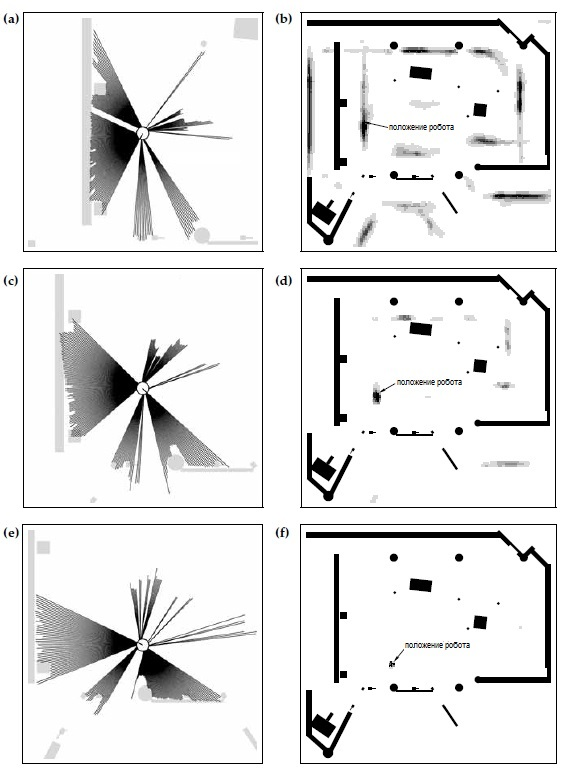
\includegraphics[width=1\linewidth]{86orig}}
	\caption{ ( Рис. 8.6 Глобальная локализация на карте с использованием лазерных датчиков расстояния.   Проход сканирования лазерных датчиков расстояния из стартовой позиции робота (максимальные показания отброшены)(a). На Рис. (b) показана ситуация после учёта результатов сканирования на равномерном распределении. Второй проход сканирования (c) и результирующая оценка (d). Учёт последнего прохода сканирования показан на Рис. (e), центр оценки у истинного положения (f). )}
	\label{fig:86orig}
\end{figure}

\begin{figure}[H]
	\center{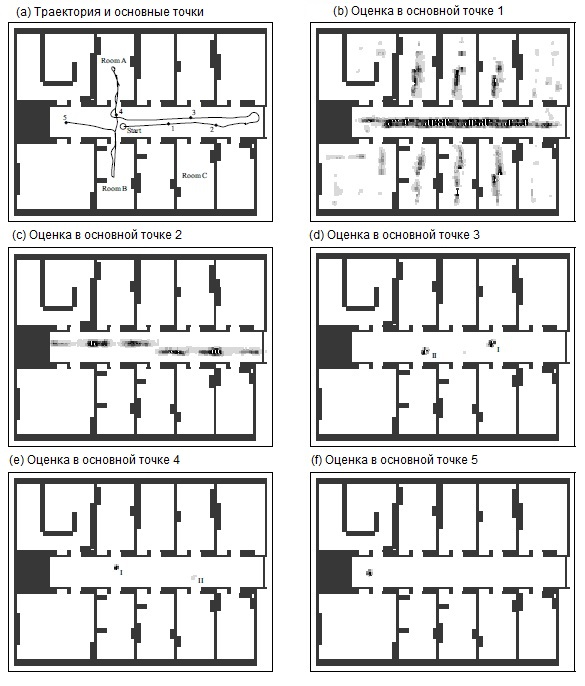
\includegraphics[width=1\linewidth]{87orig}}
	\caption{ ( Рис. 8.7  Глобальная локализация в среде офиса, на основе данных сонара.   Траектория робота(a). Оценка при прохождении роботом позиции 1 (b). После прохождения нескольких метров робот обнаруживает, что находится в коридоре (c). При достижении позиции 3 сонарами обнаруживается торец коридора и распределение концентрируется на двух локальных максимумах (d). Хотя максимум, отмеченный I отображает истинную позицию робота, из-за симметрии коридора возникает второй максимум (положение II повёрнуто на $180^\circ$ относительно положения I). После перемещения через Комнату A, вероятность нахождения в верной позиции I выше по сравнению с позицией II (e). Наконец, оценка робота концентрируется у верной позиции (f).)}
	\label{fig:87orig}
\end{figure}

\begin{figure}[H]
	\center{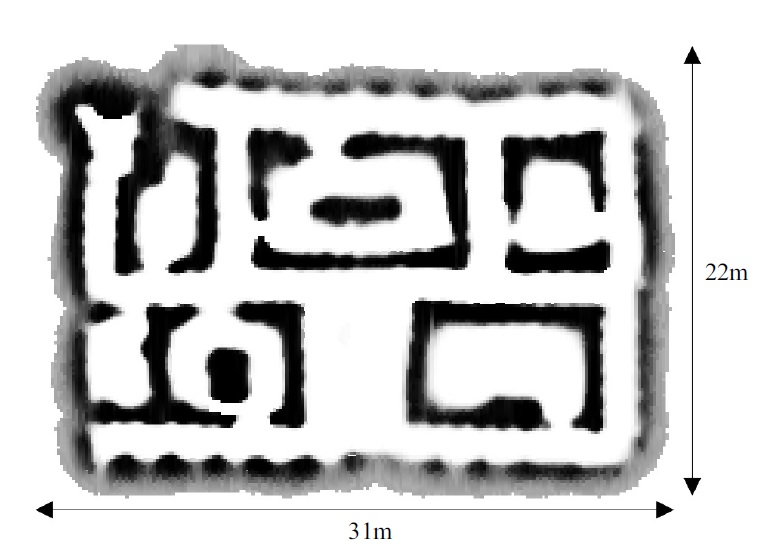
\includegraphics[width=0.9\linewidth]{88orig}}
	\caption{ ( Рис. 8.8 Карта сетки занятости соревновательной зоны для мобильных роботов конкурса AAAI 1994.)}
	\label{fig:88orig}
\end{figure}

Карта сетки занятости показана на Рис. 8.8. На Рис. 8.9a изображён набор данных, полученных при передвижении по одному из коридоров и повороте в другой. Каждый из лучей измерений на Рис. 8.9a соответствует измерению сонара. В данной конкретной среде стены гладкие и значительная часть измерений искажена. В примере снова использована вероятностная модель показаний датчиков на основе лучей, описанная в разделе 6.3. На Рис. 8.9 дополнительно показана оценка для трёх различных моментов времени, обозначенных как “A,” “B,” и “C” (Рис. 8.9a). После перемещения примерно на три метра, в течение которых робот выполнил 5 сканирований сонаром, оценки распределены почти равномерно по всем коридорам сравнительно одинакового размера, как показано на Рис 8.9b. Несколько секунд спустя оценка была разделена на несколько отдельных гипотез, как показано на Рис. 8.9c. Наконец, когда робот свернул за угол и достиг точки с меткой “C,” данных датчиков оказалось достаточно для определения уникальной позиции робота. Оценка, показанная на Рис. 8.9d, сосредоточена около настоящего положения робота. Этот пример показывает, что представление в виде сетки хорошо работает и для сильно зашумлённых данных сонара и симметричных сред, в которых при глобальной локализации необходимо поддерживать несколько гипотез. 

На Рис. 8.10 показана возможность сеточных методов корректировать накопившиеся ошибки измерений путём сравнения данных сонара с картами сеток занятости. На Рис. 8.10a показаны «сырые» данные одометрии после прохождения по траектории длиной 240 м. Очевидно, ошибка вращательного движения быстро возрастает. После прохода всего 40 м суммарная ошибка ориентации по направлению (по данным одометрии) составляет около 50 градусов. На Рис. 8.10b показан путь, пройденный роботом, согласно алгоритму локализации.

\begin{figure}[H]
	\center{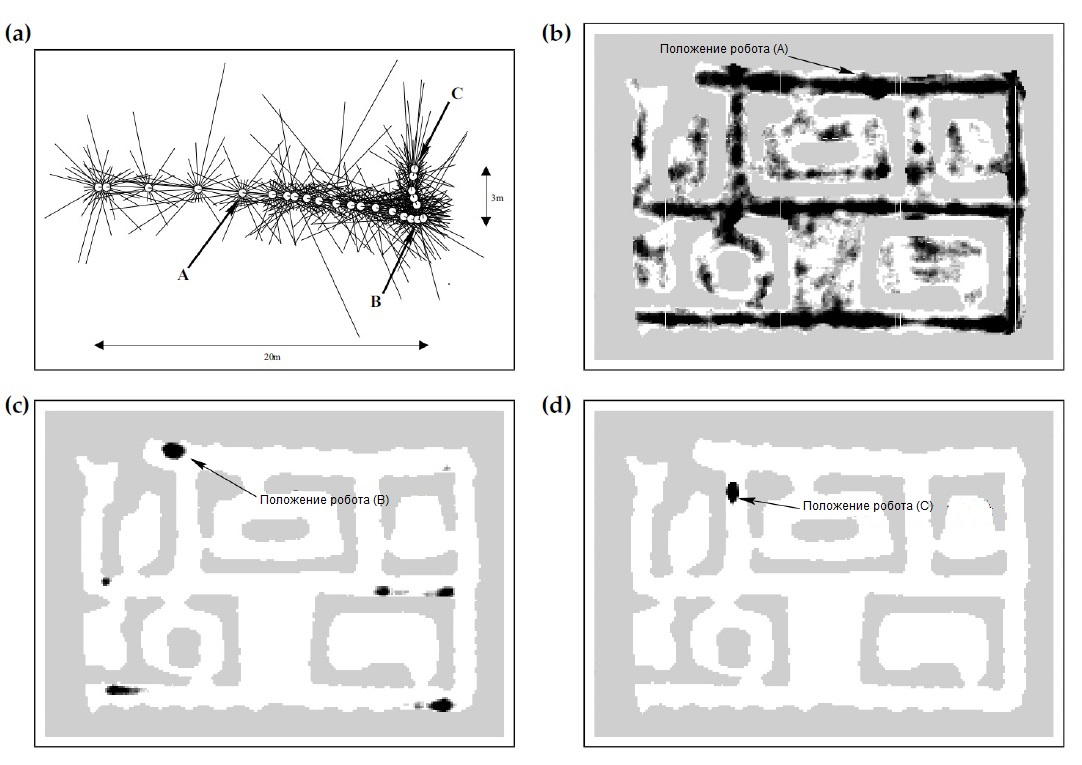
\includegraphics[width=0.9\linewidth]{89orig}}
	\caption{ ( Рис. 8.9 (a) Набор данных (одометрия и данные сканирования расстояний сонаром) собранные в среде, показанной на Рис. 8.8. Этого набора данных достаточно для глобальной локализации методом локализации по сетке. Оценки в точках, обозначенных “A”, “B” и “C” показаны на рис (b), (c) и (d).)}
	\label{fig:89orig}
\end{figure}

Очевидно, разрешение дискретного представления является ключевым параметром для марковской локализации по сетке. При наличии достаточных вычислительных ресурсов и необходимого объёма памяти, подходы с мелким разбиением обычно предпочтительнее. Как уже обсуждалось в подразделе 2.4.4, отображение в виде гистограмм вызывает систематическую ошибку, которая способна нарушить марковское свойство в фильтрах Байеса. Чем мельче разбиение, тем меньше вызываемая ошибка и лучше результаты.\\
КАТАСТРОФИЧЕСКИЙ СБОЙ\\
 Аппроксимации с мелким разбиением также менее страдают от \textit{катастрофических сбоев} при которых оценка робота существенно отличается от истинной позиции.

\begin{figure}[H]
	\center{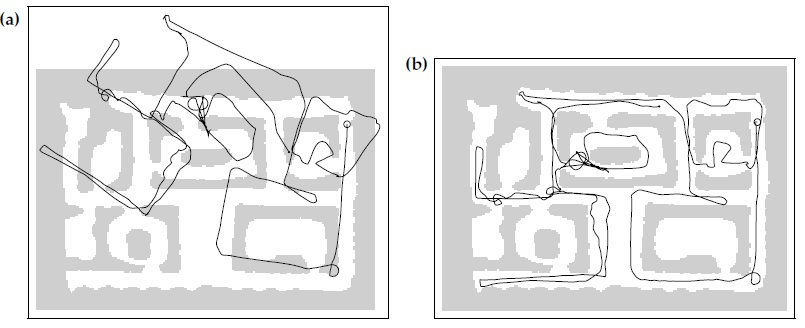
\includegraphics[width=0.9\linewidth]{810orig}}
	\caption{ ( Рис. 8.10   (a) Данные одометрии и (b) скорректированный путь робота.)}
	\label{fig:810orig}
\end{figure}

\textbf{8.3	Локализация методом Монте-Карло}\\

Теперь рассмотрим популярный алгоритм локализации, в котором  оценка $bel(x_t)$ выражена с помощью частиц. Алгоритм называется \textit{локализация методом Монте-Карло} (Monte Carlo Localization – MCL). Так же, как и марковская локализации по сетке, MCL применим как для локальной, так и для глобальной локализации. Несмотря на относительную новизну, MCL уже стал одним из самых популярных алгоритмов локализации в робототехнике. Его легко реализовать, и он хорошо работает для широкого круга проблем локализации. \\

\textbf{8.3.1	Иллюстрация}\\

На Рис. 8.11 показан MCL на примере одномерного коридора. Начальная глобальная неопределённость достигается с помощью набора частиц положений, извлекаемых случайно и равномерно из всего пространства положений, как показано на Рис. 8.11a. Когда робот обнаруживает дверь, MCL назначает каждой частице факторы значимости. Результирующий набор частиц показан на Рис. 8.11b. Высотой каждой частицы на рисунке обозначен ее вес значимости. Важно заметить, что этот набор частиц идентичен показанному на Рис. 8.11a, и единственное изменение после обновления измерения - это назначение весов. 

На. Рис. 8.11c показан набор частиц после перевыборки и учёта перемещения робота. Результатом является новый набор частиц с равномерными весами значимости, но большим количеством частиц из областей около трёх наиболее вероятных местоположений. Новое измерение назначает набору неравномерные веса значимости, как показано на Рис. 8.11d. В этой точке большинство суммарной массы вероятности сосредоточено около второй двери, которая и является наиболее вероятным местоположением. Дальнейшее перемещение вызывает ещё один такт перевыборки, и генерацию нового набора частиц согласно модели движения (Рис. 8.11e). Как очевидно из примера, выполняется приближение верной апостериорной вероятности по аналогии с точным байесовским фильтром.

\begin{figure}[H]
	\center{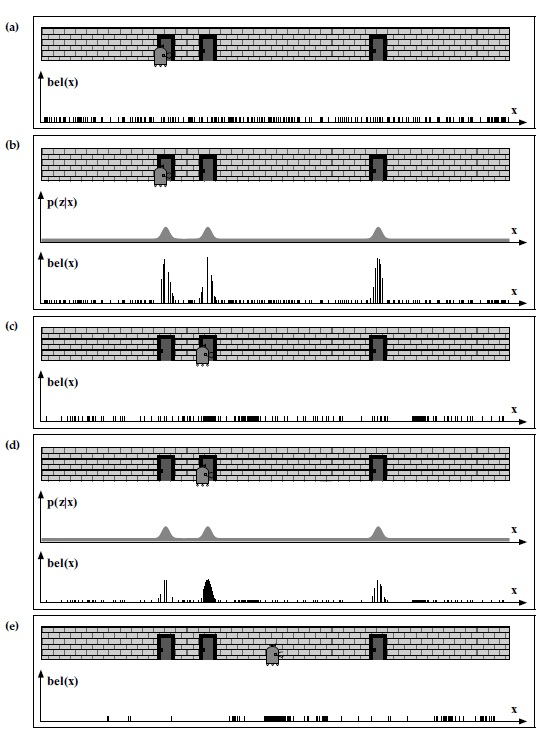
\includegraphics[width=1\linewidth]{811orig}}
	\caption{ ( Рис. 8.11 Локализация методом Монте-Карло, многочастичный фильтр в применении к задаче локализации.)}
	\label{fig:811orig}
\end{figure}

\begin{table}[H]
\begin{center}
\begin{tabular}{|l|}
\hline
{}\\
1: \textbf{Algorithm MCL}$(\mathcal{X}_{t-1},u_t,z_t,m):$ \\
2:\hspace{3mm}$\bar{\mathcal{X}}_t=\mathcal{X}_t=\emptyset$\\
3:\hspace{3mm}$\textit{for}\,m=1\,\textit{to}\,M\,\textit{do} $\\
4:\hspace{7mm}$x_t^{[m]}=\text{\textbf{sample\_motion\_model}}(u_t,x_{t-1}^{[m]})$\\
5:\hspace{7mm}$w_t^{[m]}=\text{\textbf{measurement\_model}}(z_t,x_t^{[m]},m)$\\
6:\hspace{7mm}$\bar{\mathcal{X}}_t=\bar{\mathcal{X}}_t+\langle x_t^{[m]},w_t^{[m]}\rangle$\\
7:\hspace{3mm}$\textit{endfor}$\\
8:\hspace{3mm}$\textit{for}\,m=1\,\textit{to}\,M\,\textit{do}$\\
9:\hspace{7mm}$\textit{draw}\,\,i\,\,\textit{with probability}\,\,\propto\,\,w_t^{[i]}$\\
10:\hspace{5mm}$\textit{add}\,\,x_t^{[i]}\,\,\textit{to}\,\,\mathcal{X}_t$\\
11:\hspace{3mm}$\textit{endfor}$\\
12:\hspace{3mm}$\textit{return}\,\mathcal{X}_t$\\
{}\\
\hline
\end{tabular}
\caption{(Таблица 8.2 MCL или локализация методом Монте-Карло. Алгоритм локализации, основанный на многочастичных фильтрах.)}
\end{center}
\end{table}

\textbf{8.3.2	Алгоритм MCL }\\

В Таблице 8.2 показан основной алгоритм MCL, полученный заменой соответствующих вероятностных моделей движения и восприятия алгоритмом \textbf{particle\_filters}(из Таблицы 4.3 на странице 98??? ). Базовый алгоритм MCL выражает оценку $bel(x_t)$ в виде набора $M$ частиц $\mathcal{X}_t=\{x_t^{[1]},x_t^{[2]},...,x_t^{[M]}\}$. В строке 4 алгоритма (Таблица 8.2) выполняется выборка значений из модели движения, используя в качестве начальной точки частицы из текущей оценки. Затем для определения весов значимости частицы в строке 5 используется модель движения. Начальная оценка $bel(x_0)$ получается в результате случайного извлечения $M$ таких частиц из априорного распределения $p(x_0)$, и назначения равномерного фактора значимости $M^{-1}$ каждой частице.  Как и в локализации по сетке, функции $\textbf{motion\_model}$ и
\textbf{measurement\_model} могут быть реализованы любой из моделей движения, представленных в Главе 5, и моделей измерения из Главы 6, соответственно.\\

\textbf{8.3.3	Физическая реализация}\\

Достаточно простой является реализация алгоритма MCL для сценария локализации на основе ориентиров, представленного в Главе 7. Для этого в строке 4 используется процедура выборки  в виде алгоритма \textbf{sample\_motion\_model \_velocity} из Таблицы 5.3. Алгоритм \textbf{land- mark\_model\_known \_correspondence}, приведённый в Таблице 6.4, предоставляет модель правдоподобия для взвешивания прогнозируемых значений, использованную в строке 5.

  Эта версия алгоритма MCL показана на Рис. 8.12. Сценарий идентичен показанному на Рис. 7.15. Для удобства иллюстрация пройденного роботом пути и измерений показаны на левой верхней схеме. На нижней схеме показана последовательность наборов значений выборки, сгенерированных алгоритмом MCL. Сплошными линиями показан реальный путь робота, точками – путь на основе данных управления, пунктиром показан средний путь, вычисленный алгоритмом MCL. Прогнозируемые наборы значений $\bar{\mathcal{X}}_t$ для разных моментов времени показаны тёмным цветом, значения $\mathcal{X}_t$ после шагов перевыборки - светло-серым. Каждый набор частиц определён в трехмерном пространстве положений, хотя показаны только $x$- и $y$-координаты каждой частицы. Математическое ожидание и ковариации этих наборов показаны на правой верхней схеме.

На. Рис. 8.13 показан результат использования MCL в настоящей  среде офиса роботом с массивом ультразвуковых датчиков расстояния. В этой версии MCL правдоподобие измерений вычисляется, используя алгоритм \textbf{beam\_range\_finder\_model}, приведённый в Таблице 6.1. На схеме показаны наборы частиц после передвижения робота на 5, 28 и 55 метров, соответственно. На третьей иллюстрации на Рис. 8.14 используется камера, направленная на потолок и модель измерений, соотносящая яркость в центре изображения с предварительно полученной картой потолка.\\

\textbf{8.3.4	Свойства MCL}

С помощью MCL возможно аппроксимировать практически любое распределение, имеющее практическую важность. Он не привязан к ограниченному набору параметрических подмножеств распределений, как в случае локализации с помощью EKF. Увеличение общего количества частиц увеличивает и точность аппроксимации. Количество частиц $M$ является параметром, позволяющим пользователю находить компромисс между точностью вычислений и необходимым для запуска MCL объёмом вычислительных ресурсов. Общая стратегия выбора $M$ состоит в выполнении выборки до получения следующей пары значений $u_t$ и $z_t$. Таким образом, реализация оказывается адаптивной по отношению к вычислительным ресурсам. Чем быстрее имеющийся процессор, тем лучше работает алгоритм локализации. Однако, как будет показано в подразделе 8.3.7, необходимо следить, чтобы количество частиц оставалось достаточно большим для предотвращения нарушения работы фильтра.

\begin{figure}[H]
	\center{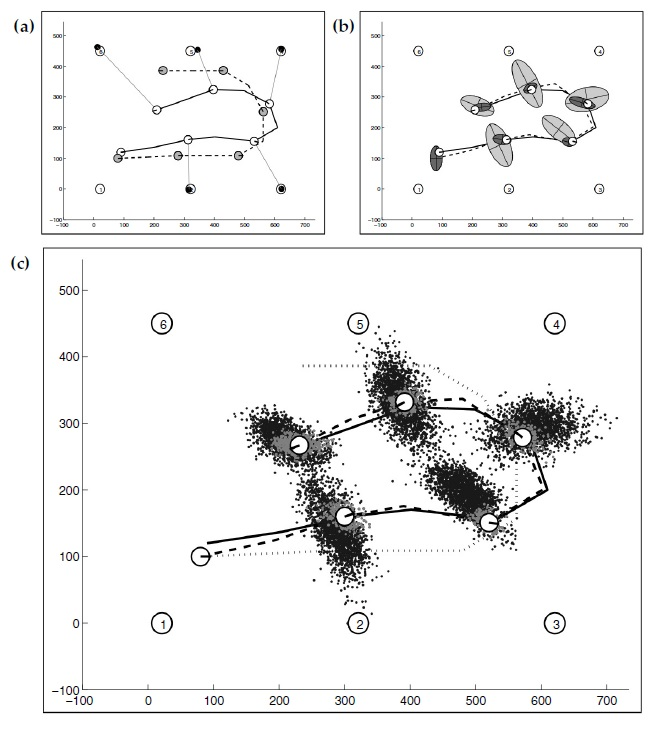
\includegraphics[width=1\linewidth]{812orig}}
	\caption{ ( Рис. 8.12 Алгоритм MCL для локализации на основе ориентиров. Траектория робота согласно управлению движением (точки) и результирующая истинная траектория (сплошная линия) (a). Обнаружение ориентиров показано тонкими линиями.  Ковариации наборов значений до и после выполнения перевыборки (b). Наборы значений до и после перевыборки (c).)}
	\label{fig:812orig}
\end{figure}

Последним преимуществом MCL является непараметрическая природа аппроксимации. Как следует из иллюстраций, с помощью MCL возможно представить сложные мультимодальные вероятностные распределения и сочетать их с сосредоточенными распределениями наподобие гауссовых функций.

\begin{figure}[H]
	\center{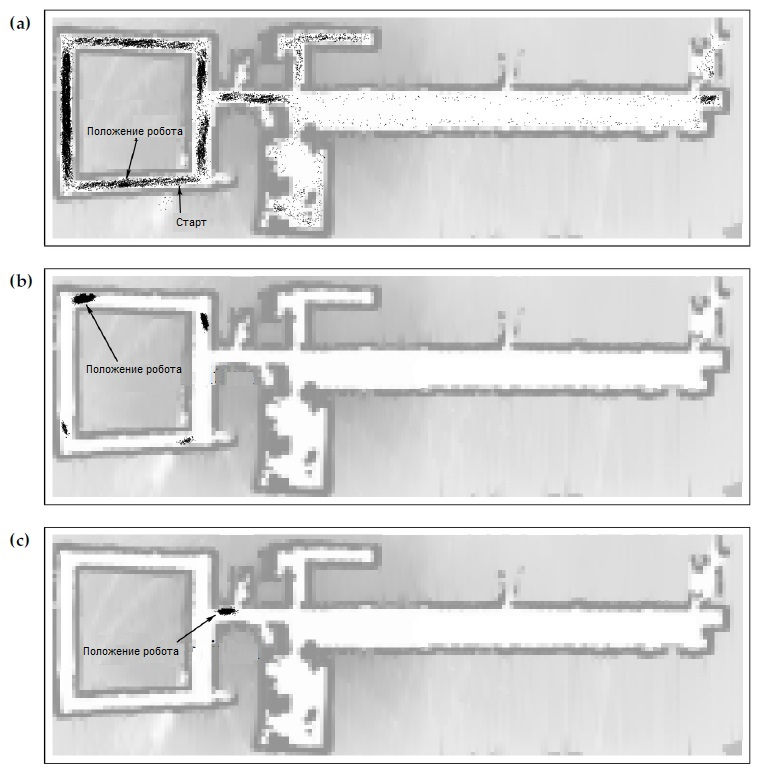
\includegraphics[width=1\linewidth]{813orig}}
	\caption{ ( Рис. 8.13 Иллюстрация локализации методом Монте-Карло. Показан робот, действующий в офисной среде размером 54 м $\times$18 м.  После перемещения на 5 м, робот все ещё неспособен определить позицию и частицы распределены на значительной части свободного пространства (a). Даже когда робот достиг левого верхнего угла карты, его оценка все ещё сосредоточена около четырёх возможных местоположений (b). Наконец, после перемещения приблизительно на 55 м, неопределённость разрешилась, и робот обнаружил, где он находится (c). Все вычисления выполнены в реальном времени на  персональном компьютере небольшой мощности.)}
	\label{fig:813orig}
\end{figure}

\begin{figure}[H]
	\center{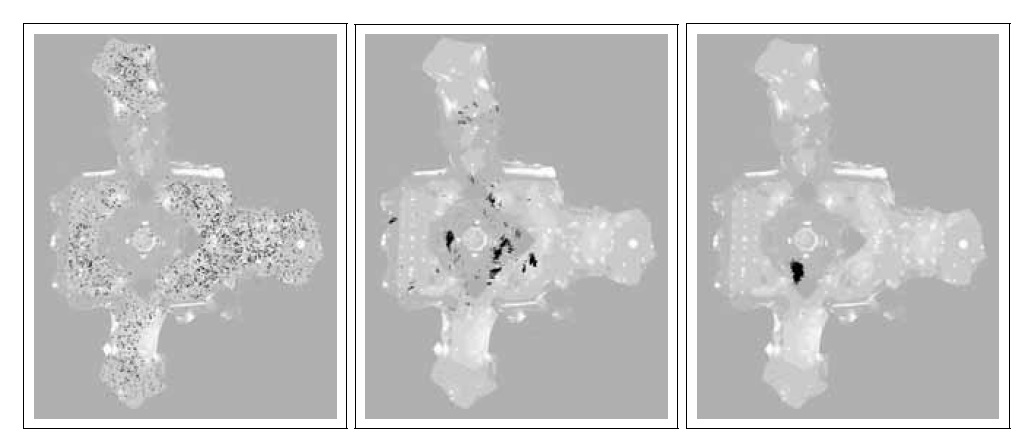
\includegraphics[width=1\linewidth]{814orig}}
	\caption{ ( Рис. 8.14    Глобальная локализация с использованием камеры, направленной на потолок.)}
	\label{fig:814orig}
\end{figure}

\textbf{8.3.5	MCL на случайных частицах: Восстановление после сбоев}\\

Алгоритм MCL в его текущем виде способен решить проблему глобальной локализации, но после сбоя «похищенного робота» или ошибок глобальной локализации восстановиться не может. Это довольно очевидно следует из результатов, показанных на Рис. 8.13. После того, как позиция определена, частицы всех положений, кроме наиболее вероятного, постепенно исчезают. В некоторый момент начинают «выживать» только частицы около единичного положения и, если это положение окажется неверным, алгоритм восстановить работу неспособен. 

Это существенная проблема и на практике в любом стохастическом алгоритме, такой как MCL, при выполнении перевыборки возможно случайное отбрасывание всех частиц вблизи верного местоположения. Эта проблема может оказаться определяющей для малого количества частиц (например, M = 50), и если частицы распределены в большом объёме, скажем, при глобальной локализации.

ВНЕСЕНИЕ СЛУЧАЙНЫХ ЧАСТИЦ

К счастью, проблему возможно решить довольно простым эвристическим методом, идея которого состоит во \textit{внесении случайных частиц} в наборы, как уже обсуждалось в подразделе 4.3.4. Такое внесение случайных частиц с математической точки зрения можно считать учётом небольшой вероятности "похищения робота" с помощью внесения в модель движения некоторой доли случайных состояний. Даже если робота не похищают, случайно добавленные частицы добавляют ещё один уровень обеспечения надёжности. 

Для метода добавления частиц возникает два вопроса. Во-первых, сколько частиц необходимо добавлять при каждой итерации алгоритма? Во-вторых, из какого распределения следует их генерировать? На первый взгляд, возможно просто добавлять некоторое фиксированное число частиц при каждой итерации, но лучше обосновать выбор некоторой оценкой работы алгоритма локализации. 

Одним из способов реализации этой идеи является мониторинг вероятности измерений датчиков \\

(8.3)
$$p(z_t|z_{1:t-1},u_{1:t},m)$$

относительно средней вероятности измерения (которую легко вычислить из данных). В многочастичных фильтрах аппроксимацию этого значения можно получить из фактора значимости, который, по определению, является стохастической оценкой вероятности. Среднее значение
\\

(8.4)
$$\frac{1}{M}\sum_{m=1}^M w_t^{[m]}\approx p(z_t|z_{1:t-1},u_{1:t},m)$$

аппроксимирует искомую вероятность. Обычно эту оценку сглаживают усреднением по нескольким тактам времени. Помимо сбоя локализации существует несколько причин низкой вероятности измерения. Так, зашумление датчика может быть чрезмерно высоким, или же на этапе глобальной локализации частицы оказываются разбросаны слишком сильно. По этим причинам предпочтительно вычислять среднее значение правдоподобия измерения в краткосрочной перспективе и соотносить его со средним значением в долгосрочной перспективе при определении числа случайных значений выборки. 

Вторую проблему определения типа распределения значений в выборке можно разрешить двумя способами. Конечно, можно извлекать частицы из пространства положений согласно однородному распределению и взвешивать их текущим измерением. 

Но для некоторых моделей датчиков возможно напрямую генерировать частицы в соответствии с распределением измерения. Одним из примеров такой модели датчика является модель обнаружения ориентиров, обсуждаемая в разделе 6.6. В этом случае дополнительные частицы могут быть напрямую помещены в местоположениях, распределенных согласно правдоподобности наблюдения (см. Таблица 6.5).

В Таблице 8.3 показан вариант алгоритма MCL с добавлением случайных частиц. Алгоритм адаптивен, поскольку отслеживает средние значения правдоподобия в краткосрочной и долгосрочной перспективе $p(z_t|z_{1:t-1},u_{1:t},m)$. Первая его часть идентична алгоритму MCL в Таблице 8.2. Новые положения извлекаются из старого набора частиц, используя модель движения (строка 5), а вес значимости для них устанавливается в соответствии с моделью измерения (строка 6).

В алгоритме \textbf{Augmented\_MCL} в строке 8 вычисляется эмпирическое правдоподобие измерения и поддерживаются средние значения правдоподобия в краткосрочной и долгосрочной перспективе в строках 10 и 11.  Для алгоритма требуется, чтобы $0\leq \alpha_{slow}\ll \alpha_{fast}$.  Параметры  $\alpha_{slow}$ и $\alpha_{fast}$, означают коэффициенты отказов экспоненциальных фильтров, выполняющих оценки средних значений в краткосрочной и долгосрочной перспективе, соответственно. Основная операция алгоритма выполняется в строке 13 -  во время процесса перевыборки случайное значение выборки будет добавлено с вероятностью\\

(8.5)
$$\max\{0.0,\,1.0-w_{fast}/w_{slow}\}$$

\begin{table}[H]
\begin{center}
\begin{tabular}{|l|}
\hline
{}\\
1: \textbf{Algorithm Augmented\_MCL}$(\mathcal{X}_{t-1},u_t,z_t,m):$ \\
2:\hspace{5mm}$\text{static}\,w_{slow},\,w_{fast}$\\
3:\hspace{5mm}$\bar{\mathcal{X}}_t=\mathcal{X}_t=\emptyset$\\
4:\hspace{5mm}$\textit{for}\,m=1\,\textit{to}\,M\,\textit{do}$\\
5:\hspace{10mm}$x_t^{[m]}=\text{\textbf{sample\_motion\_model}}(u_t,x_{t-1}^{[m]})$\\
6:\hspace{10mm}$w_t^{[m]}=\text{\textbf{measurement\_model}}(z_t,x_t^{[m]},m)$\\
7:\hspace{10mm}$\bar{\mathcal{X}}_t=\bar{\mathcal{X}}_t+\langle x_t^{[m]},w_t^{[m]}\rangle$\\
8:\hspace{10mm}$w_{avg}=w_{avg}+\frac{1}{M}w_t^{[m]}$\\
9:\hspace{5mm}$\textit{endfor}$\\
10:\hspace{4mm}$w_{slow}=w_{slow}+\alpha_{slow}(w_{avg}-w_{slow})$\\
11:\hspace{4mm}$w_{fast}=w_{fast}+\alpha_{fast}(w_{avg}-w_{fast})$\\
12:\hspace{4mm}$\textit{for}\,m=1\,\textit{to}\,M\,\textit{do}$\\
13:\hspace{9mm}$\textit{с вероятностью}\,\,\max\{0.0,\,1.0-w_{fast}/w_{slow}\}\,\,\textit{do}$\\
14:\hspace{14mm}$\textit{добавить случаное положение к}\mathcal{X}_t$\\
15:\hspace{9mm}$\textit{else}$\\
16:\hspace{14mm}$\textit{draw}\,\,i\in\{1,...,N\}\textit{с вероятностью}\,\,\propto\,\,w_t^{[i]}$\\
17:\hspace{14mm}$\textit{add}\,\,x_t^{[i]}\,\,\textit{to}\,\,\mathcal{X}_t$\\
18:\hspace{9mm}$\textit{endwith}$\\
19:\hspace{4mm}$\textit{endfor}$\\
20:\hspace{4mm}$\textit{return}\,\mathcal{X}_t$\\
{}\\
\hline
\end{tabular}
\caption{(Таблица  8.3  Адаптивный вариант алгоритма MCL с добавлением случайных значений выборки. Количество случайных значений определено сравнением правдоподобия измерений датчика в краткосрочной и долгосрочной перспективе. )}
\end{center}
\end{table}

В остальном, процесс перевыборки протекает обычным образом. В вероятности добавления случайного значения учитывается разница между средними значениями правдоподобия измерения в краткосрочной и долгосрочной перспективе. Если правдоподобие в краткосрочной перспективе лучше или равно правдоподобию в долгосрочной перспективе, случайные значения не добавляются. Если правдоподобие в краткосрочной перспективе хуже, случайные частицы добавляются пропорционально коэффициенту отношения правдоподобия. Таким образом, неожиданное отклонение правдоподобия измерения вызывает увеличение количества случайных значений. Экспоненциальное сглаживание предотвращает опасность ошибочной интерпретации мгновенного всплеска шумов датчика как плохого результата локализации. 

На Рис. 8.16 показано практическое использование дополненного алгоритма MCL на примере последовательности наборов частиц для глобальной и повторной локализации шагающего робота, оборудованного цветной камерой и действующего на поле размером $3\times2$ м, такого же, как используемое на соревнованиях по футболу RoboCup. Измерения датчиков, соответствующие обнаружению и относительной локализации шести визуальных маркеров, размещённых вокруг поля показаны на Рис. 7.7 на странице 210 ???. Алгоритм, описанный в Таблице 6.4, используется для определения правдоподобия обнаружения. Шаг 14 на Рис. 8.3 заменяется алгоритмом выборки по последнему измерению датчика и легко реализуется, используя  метод \textbf{sample\_landmark\_model\_known\_correspondence} в Таблице 6.5.

На схемах с (a) до (d) на Рис. 8.16 показана глобальная локализация. При первом обнаружении маркера практически все частицы извлекаются согласно текущему обнаружению (Рис. 8.16b). Этот этап соответствует ситуации, когда средняя вероятности измерения много хуже соответствующего долгосрочного показателя. После ещё нескольких обнаружений ориентиров частицы концентрируются вокруг истинной позиции робота (Рис. 8.16d), и возрастают как краткосрочное, так и долгосрочное среднее правдоподобие измерения. На этом этапе локализации робот только отслеживает свою позицию, правдоподобия измерений достаточно высоки и лишь иногда добавляется небольшое количество частиц. 

Когда рефери физически перемещает робота в другое место, что часто происходит на соревнованиях по футболу для роботов, вероятность измерения падает. Первое обнаружение маркера в новом местоположении пока не добавляет частиц, поскольку сглаженная оценка $w_{fast}$ все ещё высока (см. Рис. 8.16e). После нескольких обнаружений маркера, наблюдаемого из нового местоположения, $w_{fast}$ падает значительно быстрее, чем $w_{slow}$, поэтому, добавляется больше случайных частиц (Рис 8.16f и 8.16g). Наконец, робот успешно выполняет повторную локализацию, как показано на Рис. 8.16h, подтверждая, тем самым, что наш дополненный алгоритм MCL действительно способен «пережить похищение».

\begin{figure}[H]
	\center{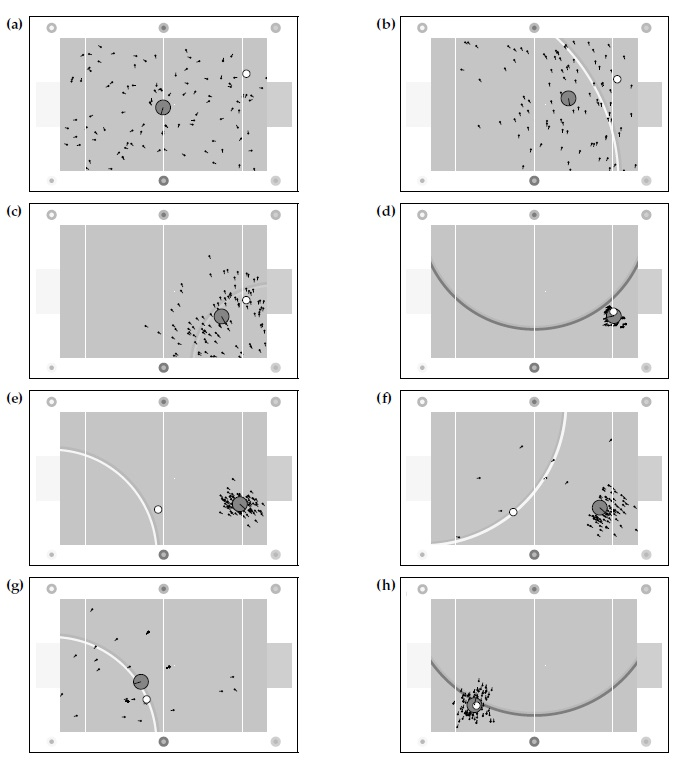
\includegraphics[width=1\linewidth]{816orig}}
	\caption{ ( Рис. 8.16 Локализация Монте-Карло со случайными частицами. На каждой картинке показан набор частиц, представляющий оценку роботом своей позиции (короткими отрезками показана ориентацию частиц). Большим кругом показано среднее оценки, истинная позиция робота обозначена маленьким белым кругом. Обнаружения маркера показаны дугами с центром в местоположении маркера. С помощью схем (a)–	(d) проиллюстрирована глобальная локализация, (e)–(h) повторная локализация. 
		)}
	\label{fig:816orig}
\end{figure}

\begin{figure}[H]
	\center{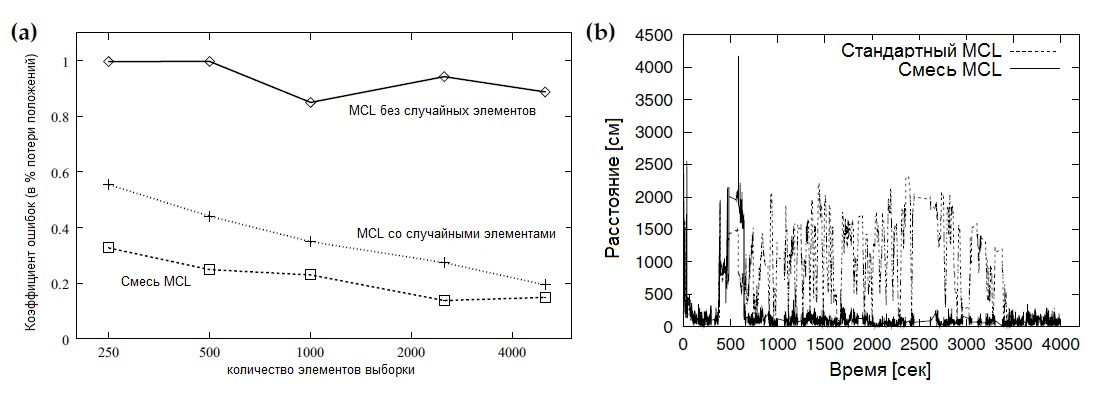
\includegraphics[width=1\linewidth]{817orig}}
	\caption{ ( Рис. 8.17 (a) базовый алгоритм MCL (верхняя кривая), MCL со случайной выборкой (центральная кривая), и смесь MCL с распределением в виде смеси (нижняя кривая). Коэффициент ошибки измерен как процент времени, в течение которого робот теряет возможность отслеживать свою позицию, для набора данных, полученных роботом, действующим в людном помещении музея. (b) Ошибка в виде функции времени для стандартного MCL и смеси MCL, при использовании для локализации карты потолка.)}
	\label{fig:817orig}
\end{figure}

\textbf{8.3.6	Модификация предполагаемого распределения}\\

Механизм предполагаемого распределения в MCL является ещё одним фактором, который может привести к неэффективности алгоритма. Как обсуждалось в подразделе 4.3.4, многочастичный фильтр использует как предполагаемое распределение модель движения, но пытается аппроксимировать произведение этого распределения и правдоподобности восприятия. Чем больше разница между предполагаемым и целевым распределениями, тем больше требуется элементов выборки. 

В алгоритме MCL это вызывает неожиданный сбой: если найти идеальный датчик, который всегда, совершенно без шумов будет выдавать роботу его истинное положение, то алгоритм MCL откажет. Это справедливо даже для идеальных датчиков, которые не несут достаточно информации для локализации. Примером может служить одномерный идеальный датчик расстояния. При получении измерения такого датчика пространство пригодных гипотез положения будет двухмерным подпространством трехмерного пространства положений робота. В подразделе 4.3.4 уже подробно обсуждалось, что шансы выборки в это двухмерное подмножество при выборке из модели движения робота равны нулю. Отсюда возникает странная ситуация, когда, при определённых обстоятельствах использования MCL для локализации, менее точный датчик будет предпочтительнее более точного. Это не так в случае локализации на основе EKF, поскольку обновление EKF принимает в расчёт измерения при вычислении нового значения средней, вместо генерации средних только лишь из модели движения. К счастью, есть простое решение. Необходимо использовать модель измерения с искусственно завышенным зашумлением датчика. Такое искусственное увеличение шумов можно воспринимать как учёт не только неопределённости измерения, но и неопределенности, вызванной приближенным характером алгоритма многочастичного фильтра. 

В альтернативном, более логичном способе решения используется модификация процесса выборки, которая уже кратко обсуждалась в подразделе 4.3.4. Идея состоит в том, чтобы инвертировать для некоторой малой частиц роли модели измерения и модели движения. Частицы, сгенерированные согласно модели измерения\\

(8.6)
$$x_t^{[m]}\sim p(z_t|x_t)$$

вес значимости для которых будет вычисляется пропорционально\\

(8.7)
$$w_t^{[m]}=\int p(x_t^{[m]}|u_t,x_{t-1})bel(x_{t-1})dx_{t-1}$$

Этот новый процесс выборки является адекватной альтернативой простому многочастичному фильтру. Но один лишь этот приём будет неэффективен, поскольку при генерации частиц полностью игнорируются предыдущие наборы. Однако, полностью применимой будет генерировать некоторую долю частиц с помощью одного из двух предложенных механизмов и объединить два набора частиц.\\
СМЕСЬ MCL\\
Результирующий алгоритм называется  \textit{MCL со смесью предполагаемых распределений}, или \textit{Смесь MCL}. На практике обычно достаточно генерировать с помощью нового процесса достаточно небольшую долю частиц (около 5\%).

К сожалению, при осуществлении этой идеи имеется ряд трудностей. Два основных шага – выборка из $p(z_t | x_t)$ и вычисление весов значимости $w_t^{[m]}$ — могут быть довольно трудны в реализации. Выборка из модели измерений легко реализуется только если её инвертированная форма имеет решение в закрытом виде, из которого легко выполняется выборка. Обычно это не так: представьте выполнение выборки из пространства всех положений, которые укладываются в сканирование расстояния лазером! Вычисление весов значимости затруднено интегралом в (8.7) и фактом того, что $bel(x_{t-1})$ само по себе представлено в виде набора частиц.

Не вдаваясь в детали, заметим, что оба шага возможно реализовать, но лишь с дополнительными приближениями. На Рис. 8.17 показаны сравнительные результаты для MCL, MCL с дополнениями случайными значениями и смеси MCL для двух реальных наборов данных. Во всех случаях $p(z_t | x_t)$ было обучено на данных и представлено деревом плотности, процедурой детализации, описание которой выходит за рамки книги. Для вычисления весов значимости интеграл был заменён стохастической интеграцией, и априорная оценка была продолжена плотностью заполнения пространства путём свёртки каждой частицы с помощью узкой гауссовой функции. Опуская детали, скажем, что это показывают лучшие результаты для идеи смеси, но может быть затруднительно для реализации.

Заметим также, что смесь MCL также позволяет логичным образом решить проблему похищенного робота. Если начать извлекать частицы, используя только самое последнее измерение, частицы будут генерироваться только в местоположениях, которые являются возможными на основании мгновенных показаний датчика, вне зависимости от предыдущих показателей управления и измерения. В литературе приводятся достаточные доказательства работоспособности таких методов для ситуации полного сбоя локализации (на Рис. 8.17b показан один такой сбой для обычного MCL), обеспечивая лучшую надёжность в практических реализациях.\\

\textbf{8.3.7	KLD-выборка: подбор размера наборов значений выборки}\\

Размер набора значений, использованного для представления оценок, является важным параметром, определяющим эффективность многочастичных фильтров. До этого момента обсуждались только многочастичные фильтры с фиксированным размером набора значений. К сожалению, чтобы избежать отклонений в работе фильтра из-за истощения набора значений в MCL, требуется выбирать большие наборы значений, чтобы позволить мобильному роботу реализовать как отслеживание положения, так и глобальную локализацию. Это может привести к растрате вычислительных ресурсов, как показано на Рис. 8.13. В этом примере все наборы значений содержат по 100000 частиц. Хотя столь большое число частиц может быть необходимым для точного представления оценки на ранних этапах локализации (см. Рис. 8.13a), очевидно, что только небольшой доли этого количества будет достаточно для отслеживания позиции, после того, как робот обнаружил своё местоположение (Рис. 8.13c).

KLD-выборка

\textit{KLD-выборка} является вариантом MCL, который меняет количество частиц со временем. Математический вывод для KLD-выборки не приводится, только алгоритм и некоторые результаты экспериментов. 

ДИВЕРГЕНЦИЯ КУЛЬБАКА-ЛЕЙБНЕРА 

Наименование "KLD-выборка" образовано из термина дивергенции Кульбака-Лейбнера, которая является мерой
разницы между двумя вероятностными распределениями. Идея KLD-выборки состоит в определении числа частиц по статистическому показателю качества аппроксимации на основе выборки. А именно, при каждой итерации многочастичного фильтра KLD-выборка определяет количество частиц таким образом, что, с вероятностью $1-\delta$, ошибка между истинным апостериорным распределением и аппроксимацией на основе выборки составляет менее $\varepsilon$. Некоторые допущения, которые здесь не приводятся, делают возможным вывод эффективной реализации. 

Алгоритм KLD-выборки показан в Таблице 8.4.  На вход принимается предыдущий набор значений, а также карта и самые последние данные управления и измерения. Зеркально по сравнению с MCL, в алгоритме KLD-выборки взвешенное значение принимается на вход. Таким образом, значения $\mathcal{X}_{t-1}$ не подвергаются перевыборке. Вдобавок, для алгоритма требуется границы статистической ошибки $\varepsilon$ и $\delta$.

В двух словах, KLD-выборка генерирует частицы, пока удовлетворяется статистическое  ограничение в строке 16. Этот порог основан на «объёме» пространства состояний, покрытого частицами. Объем, покрытый частицами, измеряется гистограммированием или сеткой, наложенной на трехмерное пространство состояний. Каждый бин гистограммы $H$ может быть или пуст, или занят, по крайней мере, одной частицей. Изначально, каждый бин установлен пустым (строки с  4 по 6). В строке 8 частица извлекается из предыдущего набора значений. На основе этой частицы прогнозируется новая частица, которая взвешивается и вставляется в новый набор значений (строки 9–11, как и в MCL).

\begin{table}[H]
\begin{center}
\begin{tabular}{|l|}
\hline
{}\\
1: \textbf{Algorithm KLD\_Sampling\_MCL}$(\mathcal{X}_{t-1},u_t,z_t,m,\varepsilon,\delta):$ \\
2:\hspace{5mm}$\mathcal{X}_t=\emptyset$\\
3:\hspace{5mm}$M=0,\,M_\chi=0,\,k=0$\\
4:\hspace{5mm}$\textit{for all}\,\,b\,\,\textit{in}\,H\,\textit{do}$\\
5:\hspace{10mm}$b=\textit{пусто}$\\
6:\hspace{5mm}$\textit{endfor}$\\
7:\hspace{5mm}$\textit{do}$\\
8:\hspace{10mm}$\textit{извлечь}\,\,i\,\,\textit{с вероятностью}\,\,\propto\,\,w_{t-1}^{[i]}$\\
9:\hspace{10mm}$x_t^{[M]}=\text{\textbf{sample\_motion\_model}}(u_t,x_{t-1}^{[i]})$\\
10:\hspace{9mm}$w_t^{[M]}=\text{\textbf{measurement\_model}}(z_t,x_t^{[M]},m)$\\
11:\hspace{9mm}$\mathcal{X}_t=\mathcal{X}_t+\langle x_t^{[M]},w_t^{[M]}\rangle$\\
12:\hspace{9mm}$\textit{if}\,\,x_t^{[M]}\textit{попадает в пустой бин \,b \,then}$\\
13:\hspace{14mm}$k=k+1$\\
14:\hspace{14mm}$b=\textit{непустой}$\\
15:\hspace{14mm}$\textit{if}\,\,k>1\,\,\textit{then}$\\
16:\hspace{16mm}$M_\chi:=\frac{k-1}{2\varepsilon}\left\lbrace 1-\frac{2}{9(k-1)}+\sqrt{\frac{2}{9(k-1)}}z_{1-\delta}\right\rbrace ^3$\\
17:\hspace{9mm}$\textit{endif}$\\
18:\hspace{9mm}$M=M+1$\\
19:\hspace{4mm}$\textit{while}\,\,M<M_\chi\,\,\textit{or}\,\,M<M_{\chi_{min}}$\\
20:\hspace{4mm}$\textit{return}\,\mathcal{X}_t$\\
{}\\
\hline
\end{tabular}
\caption{(Таблица 8.4 KLD-выборка алгоритма MCL с переменным размером набора значений. Алгоритм генерирует значения до тех пор, пока не будет достигнут статистический порог ошибки аппроксимации.  )}
\end{center}
\end{table}

В строках с 12 по 19 реализуется ключевая идея KLD-выборки. Если вновь сгенерированные частицы попадают в пустой бин гистограммы,
то количество $k$ непустых бинов увеличивается на единицу, и бин маркируется непустым. Таким образом, $k$ измеряет число бинов гистограммы, заполненных, по крайней мере, одной частицей. Это число играет важную роль в определении статистического порога в строке 16. Количество $M_\chi$ обозначает число частиц, необходимых для достижения этого порога. Заметим, что для данного $\varepsilon$, $M_\chi$, в основном, линейно зависит от числа $k$ непустых бинов. Второй, нелинейный член выражения становится пренебрежимо малым по мере возрастания $k$. Параметр $z_{1-\delta}$ основан на значении $\delta$ и выражает верхний $1-\delta$ квантиль стандартного нормального распределения. Значения $z_{1-\delta}$ для типичных значений $\delta$ доступны в стандартных статистических таблицах.

Алгоритм генерирует новые частицы до тех пор, пока их число $M$ не превысит $M_\chi$ и определённый пользователем минимум $M_{\chi_{min}}$. Как можно увидеть, порог $M_\chi$ служит «движущейся мишенью» для $M$. Чем больше элементов выборки $M$ генерируется, тем больше бинов $k$ в гистограмме не пусты и тем выше порог $M_\chi$.

На практике алгоритм прерывает работу по следующим причинам. На начальных этапах выполнения выборки значение $k$ возрастает практически с каждым новым элементом, поскольку почти все бины пусты. Это увеличение значения $k$ приводит к увеличению порога $M_\chi$. Однако, со временем заполняется все больше и больше бинов, а $M_\chi$ возрастает достаточно редко. Поскольку $M$ увеличивается с каждым новым элементом, $M$ в какой-то момент достигнет $M_\chi$, и процесс выборки остановится. Момент, когда это произойдет, зависит от оценки. Чем более разбросаны частицы, тем больше бинов заполнены и тем выше порог $M_\chi$. При операции отслеживании KLD-выборка генерирует меньше элементов, поскольку частица сконцентрированы на небольшом числе разных бинов. Следует заметить, что гистограмма не оказывает никакого влияния на само распределение частиц и её единственное назначение – измерять сложность, или объем оценки. В конце каждой итерации многочастичного фильтра сетка отбрасывается.

Рис. 8.18 показаны размеры наборов значений для типичного примера глобальной локализации, используя KLD-выборку. На рисунке приведены схемы использования лазерного датчика расстояния (сплошная линия) и ультразвуковых датчиков (пунктирная линия). В обоих случаях алгоритм отбирает большое количество значений на начальном этапе глобальной локализации. Когда локализация робота завершена, количество частиц уменьшается до гораздо более низкого уровня (менее 1\% от начального числа частиц). В какой момент и насколько быстро произойдёт переход от глобальной локализации к отслеживанию позиции зависит от типа среды и точности датчиков. В данном примере более высокая точность лазерных датчиков расстояния повлекла более ранний переход на низший уровень.

\begin{figure}[H]
	\center{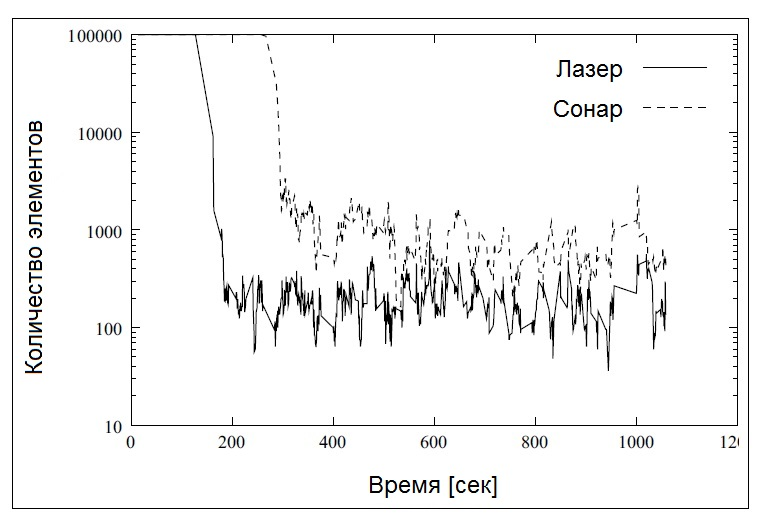
\includegraphics[width=0.8\linewidth]{818orig}}
	\caption{ ( Рис. 8.18 KLD-выборка. Типичное изменение количества элементов для прохода глобальной локализации, на графике по времени (количество элементов показано на логарифмической шкале). Сплошной линией показано количество элементов при использовании лазерного датчика расстояния,  пунктиром - данные сонара.)}
	\label{fig:818orig}
\end{figure}

На Рис. 8.19 показана разница между ошибкой аппроксимации KLD- выборки и MCL с фиксированным размером наборов значений. Ошибка аппроксимации измерена с помощью расстояния Кульбака-Лейбнера между оценками (наборами элементов), сгенерированных с различным числом элементов и «оптимальными» оценками. Эти «оптимальные» оценки были сгенерированы запуском MCL с наборами из 200000 элементов, которых более чем достаточно для оценки позиции. Как и ожидалось, чем больше значений использовано, тем меньше ошибка аппроксимации. На пунктирном графике показаны результаты, полученные с помощью MCL с разным размером наборов значений. Как можно увидеть, для фиксированного метода требуется около 50000 элементов, прежде чем он перейдет к расстоянию KL менее 0,25. Большие значения обычно указывают на расхождение многочастичного фильтра и неспособность робота выполнить локализацию. Сплошной линией показаны результаты использования KLD-выборки с размерами наборов элементов усреднённых по проходам глобальной локализации. Различные точки данных были получены изменением порога ошибки $\varepsilon$ в диапазоне от 0,4 до 0,015, изображённой на графике по убывающей слева направо. KLD-выборка переходит на малый уровень ошибки, используя только около 3000 значений. На графике также показано, что KLD-выборка не гарантирует точного отслеживания оптимальной оценки. Самые левые точки данных на сплошной линии указывает, что KLD-выборка разошлась из-за слишком больших пороговых параметров.

\begin{figure}[H]
	\center{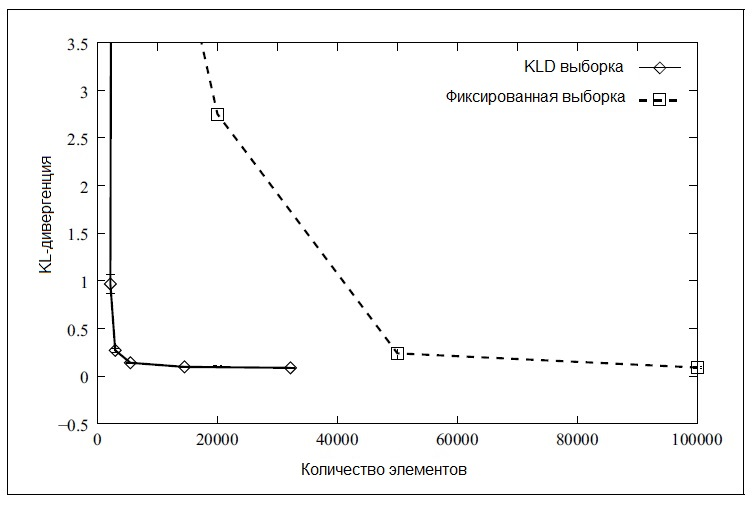
\includegraphics[width=0.8\linewidth]{819orig}}
	\caption{ ( Рис. 8.19 Сравнение KLD-выборки и MCL с фиксированным размером наборов элементов.  По оси $x$ показаны средние размеры наборов элементов. По оси $y$ показаны графики KL-расстояния между эталонными оценками и наборами элементов, сгенерированных двумя методами.)}
	\label{fig:819orig}
\end{figure}

KLD-выборка может использоваться в любом многочастичном фильтре, не только в MCL. Гистограмма может быть реализована как в виде фиксированной многомерной сетки, так и в более компактных древовидных структурах. В контексте локализации робота было показано, что KLD-выборка стабильно превосходит MCL с фиксированным размером наборов элементов. Преимущество этого метода наиболее существенно для сочетания глобальной локализации и отслеживания. На практике хорошие результаты достигаются при пороговых значениях ошибки около 0,99 для $(1-\delta)$ и 0,05 для $\varepsilon$ в сочетании с размерами бинов гистограммы  50 см$\times$50 см $\times$15 градусов.\\

\textbf{8.4	Локализация в динамических средах}\\

Ключевое ограничение всех обсуждаемых алгоритмов локализации возникает в силу условности о статической природе среды или марковского свойства. Наиболее интересные для роботов среды населены людьми и, поэтому, имеют динамику, которую не удаётся моделировать состоянием $x_t$. До некоторой степени вероятностные подходы устойчивы к такой несмоделированной динамике из-за способности приспосабливаться к шумам датчиков. Однако, как было указано ранее, шум датчика, который возможно обработать вероятностными алгоритмами фильтров, должен быть независимым на каждом такте времени, в то время, как несмоделированная динамика вызывает воздействие на измерения датчика продолжительностью несколько тактов времени. Когда такие эффекты сохраняются, вероятностные алгоритмы локализации, основанные на допущении о статической среде, могут отказывать. 

Хороший пример такой ситуации отказа показан на Рис. 8.20. В этом примере использован мобильный робот-экскурсовод, выполняющий навигацию в музее, полном людей. Люди, а точнее их местоположение, скорости и намерения перемещения являются скрытыми состояниями для алгоритма локализации и не обнаруживаются методами, которые обсуждались ранее. Почему это является проблематичным? Представим, что люди расположились таким образом, что робот ошибочно принял их за стену. С каждым новым измерением датчика оценка робота о том, что он находится у стены, возрастает. Поскольку информация считается независимой, назначается более высокое правдоподобие для положений около стен. Такой эффект возможен и для независимого шума датчика, на правдоподобие в этом случае будет исчезающе мало.

\begin{figure}[H]
	\center{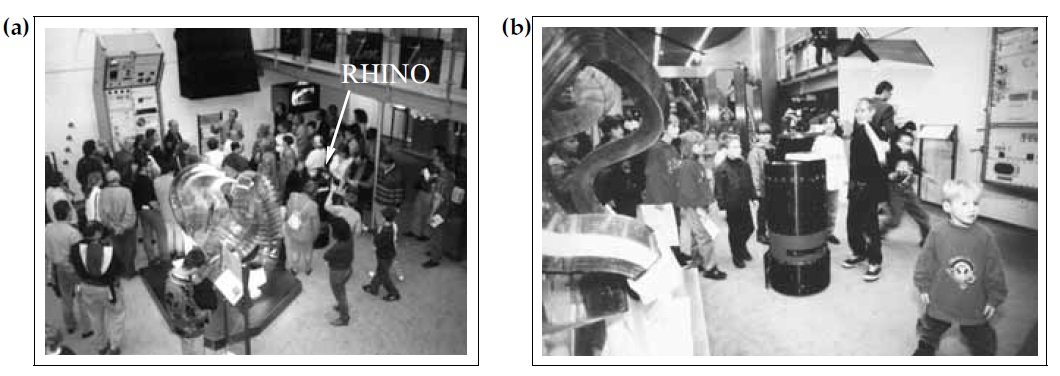
\includegraphics[width=1\linewidth]{820orig}}
	\caption{ ( Рис. 8.20 Сцены из \textit{“Deutsches Museum Bonn,”} в которых мобильный робот «Рино» (“Rhino”) часто находился в окружении десятков людей.)}
	\label{fig:820orig}
\end{figure}

\begin{figure}[H]
	\center{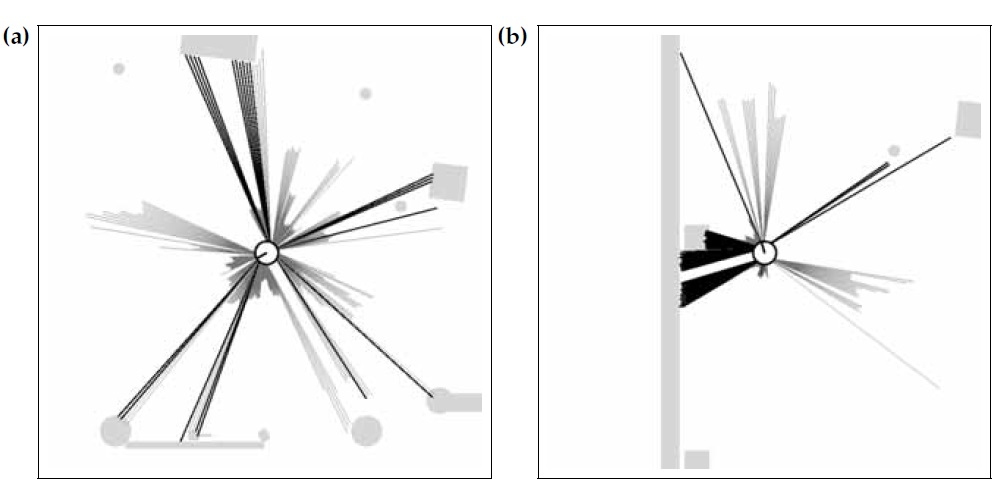
\includegraphics[width=1\linewidth]{821orig}}
	\caption{ ( Рис. 8.21 Показания лазерного датчика расстояния часто были сильно повреждены, когда люди находились вокруг робота. Как робот может выполнить точную локализацию в такой ситуации?)}
	\label{fig:821orig}
\end{figure}

ДОПОЛНЕНИЕ СОСТОЯНИЯ\\

Существуют два фундаментальных метода для работы с динамическими средами. Первый метод, \textit{дополнение состояния}, включает скрытое состояние в состояние, оцениваемое фильтром.  Другой, \textit{отбрасывание выбросов} предварительно обрабатывает измерения датчика для удаления искажённых измерений. Вторая технология является математически более обобщённой: вместо простой оценки положения робота, можно определить фильтр для оценки положения людей, их скоростей и так далее. Позже мы обсудим такой подход, как расширение алгоритма картографирования мобильного робота.

Принципиальный недостаток оценивания переменных скрытого состояния состоит в вычислительной сложности. Вместо оценки 3 переменных необходимо вычислять апостериорные распределения для значительно большего количества переменных. Фактически, количество переменных само является переменной величиной, поскольку количество переменных со временем меняется. Поэтому, результирующий алгоритм будет существенно более сложным, чем алгоритмы локализации, которые обсуждались до настоящего момента.

ОТБРАСЫВАНИЕ ВЫБРОСОВ

Альтернативный подход, \textit{отбрасывание выбросов}, хорошо работает в некоторых ограниченных случаях, например, когда присутствие людей может влиять на датчики расстояния или, в меньшей мере, на изображения с камер. Далее будет показан алгоритм для модели датчика расстояния на основе лучей из раздела 6.3.

Идея состоит в том, чтобы найти причину конкретного измерения датчика и и отбросить искажённые несмоделированной динамикой окружающей среды. Обсуждаемые модели датчиков используют самые разнообразные способы того, как может появиться измерение. Если мы сумеем связать конкретные способы появления измерения с присутствием нежелательных эффектов динамики (например, людей), то останется только отбросить измерения с высоким правдоподобием для несмоделированных сущностей. 

Идея носит удивительно обобщенный характер и основывается на той же математике, что и в \textit{алгоритме обучения EM }в разделе 6.3, но в онлайновом варианте. В Уравнении (6.12) в разделе 6.3 была определена модель измерения на основе лучей для датчиков расстояния в виде смеси четырех составляющих:

(8.8)
\begin{minipage}{0.2\textwidth}
	\begin{equation*}
	p(z_t^k|x_t,m)=
	\left(\begin{array}{c}
	z_{hit}\\
	z_{short}\\
	z_{max}\\
	z_{rand}\\
	\end{array}\right)^T
	\cdot
	\left(\begin{array}{c}
	p_{hit}(z_t^k|x_t,m)\\
	p_{short}(z_t^k|x_t,m)\\
	p_{max}(z_t^k|x_t,m)\\
	p_{rand}(z_t^k|x_t,m)\\
	\end{array}\right)
	\end{equation*}
\end{minipage}\\

Как видно при выводе модели, один из членов выражения, включающий $z_{short}$ и $p_{short}$, соответствует незапланированным объектам. Для вычисления вероятности того, что измерение $z_t^k$ соответствует незапланированному объекту введём новую переменную соответствия, $\bar{c}_t^k$ которая может принимать одно из четырёх значений \{отражение, близко, максимально далеко, случайно\}.
 
Апостериорная вероятность того, что измерение $z_t^k$ соответствует показанию «близко» (нашему обозначению незапланированного препятствия из раздела 6.3) получается применением теоремы Байеса и последовательным отбрасыванием нерелевантных переменных:\\

(8.9)
\begin{equation*}
\begin{split}
p(\bar{c}_t^k&=\text{short}|z_t^k,z_{1:t-1},u_{1:t},m)\\
&=\frac{p(z_t^k|\bar{c}_t^k=\text{short},z_{1:t-1},u_{1:t},m)\,\,p(\bar{c}_t^k=\text{short}|z_{1:t-1},u_{1:t},m)}{\sum_c p(z_t^k|\bar{c}_t^k=c,z_{1:t-1},u_{1:t},m)\,\,p(\bar{c}_t^k=c|z_{1:t-1},u_{1:t},m)}\\
&=\frac{p(z_t^k|\bar{c}_t^k=\text{short},z_{1:t-1},u_{1:t},m)\,\,p(\bar{c}_t^k=\text{short})}{\sum_c p(z_t^k|\bar{c}_t^k=c,z_{1:t-1},u_{1:t},m)\,\,p(\bar{c}_t^k=c)}
\end{split}
\end{equation*} 
 
Здесь переменная $c$ в знаменателе принимает одно из четырёх значений \{отражение, близко, далеко, случайно\}. Используя нотацию выражения (8.8), априорная вероятность $p(\bar{c}_t^k=c)$ задана переменными $z_{hit}$, $z_{short}$, $z_{max}$ и $z_{rand}$ для четырёх указанных значений $c$. Оставшаяся вероятность в (8.9) получается интегрированием $x_t$:\\

(8.10)
\begin{equation*}
\begin{split}
p(z_t^k|\bar{c}_t^k&=c,z_{1:t-1},u_{1:t},m)\\
&=\int p(z_t^k|x_t,\bar{c}_t^k=c,z_{1:t-1},u_{1:t},m)\,\,p(x_t|\bar{c}_t^k=c,z_{1:t-1},u_{1:t},m)dx_t\\
&=\int p(z_t^k|x_t,\bar{c}_t^k=c,m)\,\,p(x_t|z_{1:t-1},u_{1:t},m)dx_t\\
&=\int p(z_t^k|x_t,\bar{c}_t^k=c,m)\,\,\overline{bel}(x_t)dx_t
\end{split}
\end{equation*} 
 
Вероятности в форме $p(z_t^k|x_t,\bar{c}_t^k=c,m)$ сокращаются по $p_{hit}$, $p_{short}$, $p_{max}$ и $p_{rand}$ аналогично разделу 6.3. Это даст выражение искомой вероятности (8.9):\\

(8.11)
$$p(\bar{c}_t^k=\text{short}|z_t^k,z_{1:t-1},u_{1:t},m)=\frac{\int p_{short}(z_t^k|x_t,m)z_{short}\overline{bel}(x_t)dx_t}{\int\sum_c p_c(z_t^k|x_t,m)z_c\overline{bel}(x_t)dx_t} $$
 
В общем, интегралы в (8.11) не имеют решений в закрытом виде. Для их оценки следует выполнить аппроксимацию репрезентативными значениями апостериорной вероятности $\overline{bel}(x_t)$ по состоянию $x_t$. Эти значения могут быть ячейками сетки с высоким правдоподобием в алгоритме локализации по сетке или частиц в алгоритме MCL. Измерение отбрасывается, если его вероятность быть вызванным незапланированным препятствием превышает определённый пользователем порог $\chi$. 
 
\begin{table}[H]
\begin{center}
\begin{tabular}{|l|}
\hline
{}\\
1: \textbf{Algorithm test\_range\_measurement}$\,(z_t^k,\bar{\mathcal{X}}_t,m):$ \\
2:\hspace{5mm}$p=q=0$\\
3:\hspace{5mm}$\textit{for}\,\,m=1\,\,\textit{to}\,M\,\textit{do}$\\
4:\hspace{10mm}$p=p+z_{short}\,\cdot\,p_{short}(z_t^k|x_t^{[m]},m)$\\
5:\hspace{10mm}$q=q+z_{hit}\,\cdot\,p_{hit}(z_t^k|x_t^{[m]},m)+z_{short}\,\cdot\,p_{short}(z_t^k|x_t^{[m]},m)$\\
6:\hspace{15mm}$+z_{max}\,\cdot\,p_{max}(z_t^k|x_t^{[m]},m)+z_{rand}\,\cdot\,p_{rand}(z_t^k|x_t^{[m]},m)$\\
7:\hspace{5mm}$\textit{endfor}$\\
8:\hspace{5mm}$\textit{if}\,\,p/q\leq\chi\,\,\textit{then}$\\
9:\hspace{10mm}$\textit{return}\,\,\text{accept}$\\
10:\hspace{4mm}$\textit{else}$\\
11:\hspace{9mm}$\textit{return}\,\,\text{reject}$\\
12:\hspace{4mm}$\textit{endif}$\\
{}\\
\hline
\end{tabular}
\caption{(Таблица 8.5   Алгоритм тестирования измерений расстояния в динамической среде.)}
\end{center}
\end{table} 
 
В Таблице 8.5 приводится реализация этого метода в контексте многочастичных фильтров.  На вход принимается набор частиц $\bar{\mathcal{X}}_t$, выражающий оценку $\overline{bel}(x_t)$ измерения расстояния $z_t^k$ и карты.  Если вероятность того, что измерение соответствует незапланированному препятствию превышает $\chi$, возвращается значение «отбросить», в противном случае возвращается «принять». Эта процедура предшествует такту интеграции измерения в MCL.

На Рис. 8.22 показан эффект фильтра. На обоих врезках показано сканирование дальности для различных соответствий с положением робота. Выделенные светлым цветом измерения превышают порог и отбрасываются. Ключевым свойством механизма отбрасывания является фильтрация измерений, которые «необычно коротки», но сохранение тех, что «необычно велики». Эта асимметрия отражает факт того, что появление людей вызывает более короткие измерения по сравнению с ожидаемыми. Принимая неожиданно длинные измерения, метод позволяет сохранять возможность восстанавливаться после сбоев глобальной локализации. 

На Рис. 8.23 показан эпизод, в котором робот передвигается в среде, где присутствует множество людей (см. Рис. 8.21). Показан также предполагаемый путь робота по всем конечным точкам, учтённым в алгоритме локализации. На рисунке показана эффективность удаления измерений, не соответствующим физическим объектам карты: на правой схеме очень мало оставшихся измерений расстояния в свободном пространстве, поскольку принимаются только измерения, превосходящие пороговое значение.

\begin{figure}[H]
	\center{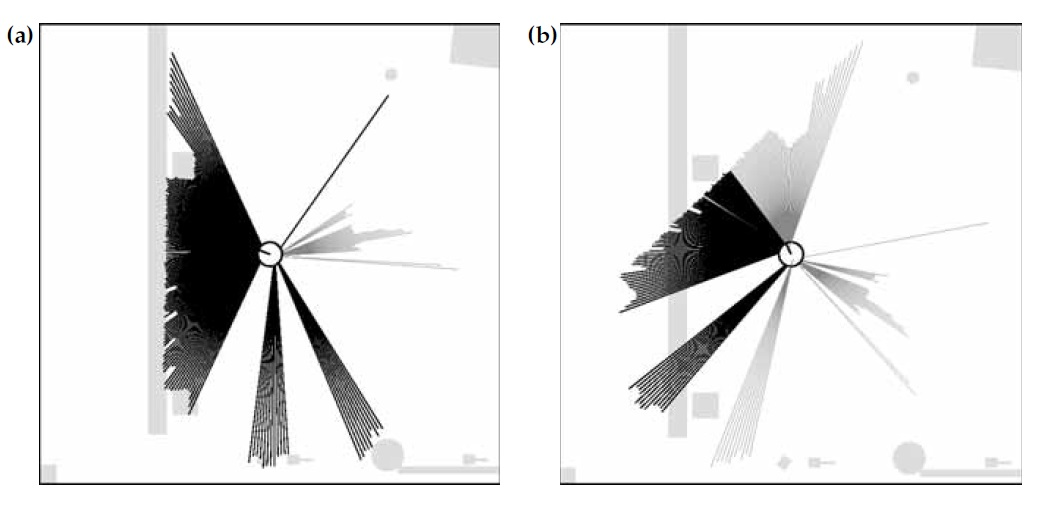
\includegraphics[width=1\linewidth]{822orig}}
	\caption{ ( Рис. 8.22 Иллюстрация алгоритма отбрасывания измерений. На обоих схемах показаны измерения расстояния (без максимальных показаний). Выделенные светлым показания отбрасываются.)}
	\label{fig:822orig}
\end{figure}

В общем случае, отбрасывание измерений является хорошей идеей. Статических сред практически не существует, поскольку даже в  условиях офиса мебель может передвигаться, двери – открываться и закрываться и так далее. Приведённая реализация использует асимметрию измерений, поскольку присутствие людей укорачивает измерения, а не удлиняет. При использовании того же метода на других данных (например, изображениях) или других типах модификации среды (например, удаление физического препятствия), такая асимметрия может не существовать. Тем не менее, тот же вероятностный анализ все же применим. Недостатком отсутствия симметрии может стать невозможность восстановления после сбоев глобальной локализации, поскольку каждое необычное измерение будет отбрасываться. В таких случаях может иметь смысл добавление новых ограничений, например, предельной доли измерений, которые считаются повреждёнными. 

Заметим, что проверка на отбрасывание применима даже в весьма статичных средах по довольно неявным причинам. Модель датчика на основе лучей прерывистая: малые изменения положения могут весьма сильно изменить апостериорную вероятность измерения датчика. Это происходит потому, что результат операции бросания лучей не является непрерывной функцией параметров положения, таких как ориентация робота по направлению. В средах с большим количеством объектов из-за этого увеличивается количество частиц, необходимых для успешной локализации. Путём ручного удаления чрезмерно загромождённых мест с карты и использования фильтра для удаления ошибочных слишком «близких» измерений число частиц можно значительно уменьшить. 

\begin{figure}[H]
	\center{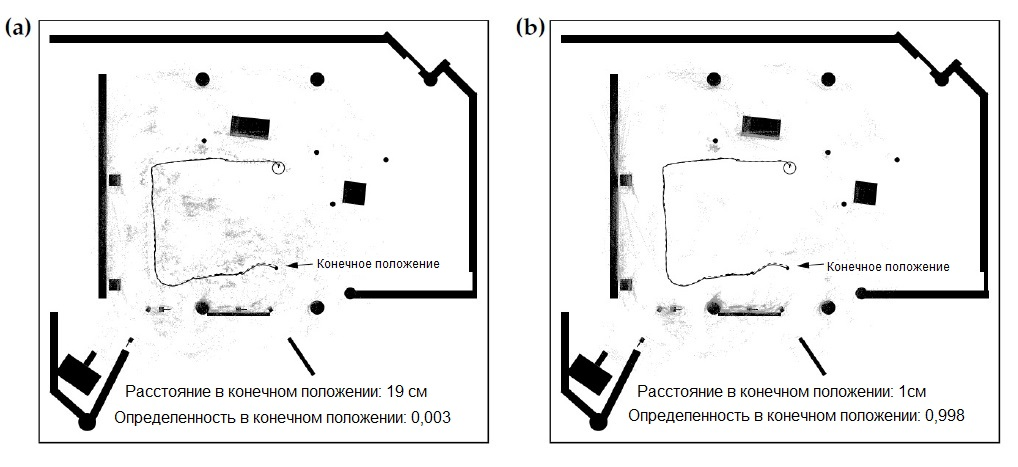
\includegraphics[width=1\linewidth]{823orig}}
	\caption{ ( Рис. 8.23 Сравнение  стандартного MCL (a) и датчика MCL с удалением измерений, которые, скорее всего, вызваны неожиданными препятствиями (b). На обоих схемах показан путь робота и конечные точки сканирования, используемые для локализации.)}
	\label{fig:823orig}
\end{figure}

Эта модель неприменима для модели полей правдоподобия, поскольку она гладкая относительно параметров положения робота.\\ 

\textbf{8.5	Практические соображения}\\

В Таблице 8.6 приводятся и сравниваются основные методы локализации, обсуждаемые в этой и предыдущих главах. При выборе метода необходимо соблюдать компромисс между различными требованиями. Первым вопросом всегда будет предпочтительность извлечения признаков из измерений датчика. Извлечение признаков может оказаться выигрышным с вычислительной точки зрения, но по цене уменьшенной точности и надёжности.

Хотя в этой главе обсуждались методы для работы в динамических средах в контексте алгоритма MCL, похожие методы могут использоваться и для других методов локализации. Фактически, представленные методы лишь иллюстрируют гораздо более обширное семейство алгоритмов. 

При реализации алгоритма локализации стоит настроить дополнительные настройки параметров. Например, условные вероятности часто увеличивают при интеграции близлежащих измерений, для учёта несмоделированных зависимостей, которые всегда присутствуют в робототехнике. Хорошим подходом является сбор эталонных наборов данных, и настойка алгоритма до получения удовлетворительных результатов. Это необходимо потому, что независимо от сложности математической модели всегда будут оставаться не моделированные зависимости и источники систематических шумов, влияющие на общий результат.   

\begin{table}[H]
\begin{center}
\begin{tabular}{|l|l|l|l|l|l|}
\hline
{}&
\text{EKF}&\text{MHT}&\text{грубая (топо- }&\text{мелкая} &\text{MCL}\\
{}&{}&{}&\text{логическая) }&\text{(метрическая)}&{}\\
{}&{}&{}&\text{сетка}&\text{сетка}&{}\\
\hline
\text{Измерения}&\text{ориентиры}&\text{ориентиры}&\text{ориентиры}&\text{исходные}&\text{исходные}\\
{}&{}&{}&{}&\text{измерения}&\text{измерения}\\
\hline
\text{Шум}&\text{гауссовы}&\text{гауссовы}&\text{любые}&\text{любые}&\text{любые}\\
\text{измерения}&{}&{}&{}&{}&{}\\
\hline
\text{апостериорное}&\text{гауссовы}&\text{смесь}&\text{гистограмма}&\text{гистограмма}&\text{частицы}\\
\text{распределение}&{}&\text{гауссианов}&{}&{}&{}\\
\hline
\text{Эффективность}&$++$&$++$&$+$&$-$&$+$\\
\text{(память)}&{}&{}&{}&{}&{}\\
\hline
\text{Эффективность}&$++$&$+$&$+$&$-$&$+$\\
\text{(время)}&{}&{}&{}&{}&{}\\
\hline
\text{Легкость}&$+$&$-$&$+$&$-$&$++$\\
\text{реализации}&{}&{}&{}&{}&
{}\\
\hline
\text{Разрешение}&$++$&$++$&$-$&$+$&$+$\\
\hline
\text{Устойчивость}&$-$&$+$&$+$&$++$&$++$\\
\hline
\text{Глобальная }&\text{нет}&\text{да}&\text{да}&\text{да}&\text{да}\\
\text{локализация}&{}&{}&{}&{}&{}\\
\hline
\end{tabular}
\caption{(Таблица 8.6   Сравнение разных реализаций марковских алгоритмов локализации.)}
\end{center}
\end{table}

\textbf{8.6	Выводы}\\

В этой главе обсуждались два семейства вероятностных алгоритмов локализации: сеточные методы и методы Монте-Карло (MCL).\\

•	Сеточные методы отображают апостериорные распределения в виде гистограмм.\\

•	Степень разбиения сетки определяется компромиссом между точностью и вычислительной эффективностью. Для грубых сеток обычно необходимо настраивать модели датчика и движения для учёта негативных эффектов разбиения. Для тонких разбиений может понадобиться выборочное обновление ячеек сетки в целях уменьшения общей вычислительной нагрузки.\\

•	Алгоритм локализации Монте-Карло отображает апостериорное распределение, в виде набора частиц. Баланс между вычислительной стоимостью и точностью достигается путём установки размера набора частиц. \\

•	И методы локализации по сетке, и MCL способны выполнять глобальную локализацию робота.\\

•	После добавления случайных частиц MCL также способны решить проблему похищенного робота.\\

•	Смесь MCL - это обобщение, инвертирующее процесс генерации частицы для некоторой части всех частиц. Это позволяет достичь улучшенной производительности для роботов с малошумными датчиками, но ценою более сложной реализации.\\

•	KLD-выборка повышает эффективность многочастичных фильтров с помощью настройки размера наборов элементов. Максимальная эффективность этого метода достигается, если сложность оценок значительно изменяется со временем.\\

•	Несмоделированная динамика среды может быть обработана фильтрацией данных датчиков, отбрасывая измерения, для которых велико правдоподобие, того, что объекту не был моделирован. При использовании датчиков расстояния робот отбрасывает показания датчиков, которые необычно малы.\\

Популярность MCL, возможно, проистекает из двух факторов. MCL является одним из самых простых в реализации алгоритмов локализации и одним из самых мощных, поскольку способен аппроксимировать практически любое распределение. \\

\textbf{8.7 Библиографические примечания}\\

Локализация Монте-Карло на основе сеток была представлена Симмонсом и Кенигом (Simmons and Koenig), на основе связанного метода поддержки факторов определенности Нурбакша (Nourbakhsh et al., 1995). После основополагающей работы Симмонса и Кенига (Simmons and Koenig, 1995) возникло большое количество методов, поддерживающих гистограммы для локализации (Kaelbling et al. 1996). Хотя в первоначальной работе были использованы достаточно грубые разбиения для решения проблемы чрезвычайно высокой вычислительной нагрузки  при обновлении сетки, Бургард (Burgard et al, 1996) предложил методы выборочного обновления, для применения сетки значительно более высокого разрешения. 
Это развитие часто рассматривалось как переход от грубой, топологической марковской локализации к детализированной метрической. Обзорные статьи об этих работах можно найти у Кенига и Симмонса (Koenig and Simmons, 1998), Фокса (Fox et al., 1999c). 

Ряд лет методы на основе сеток считались наиболее совершенными для локализации мобильного робота и возможно найти множество различных примеров успешных реализаций марковской локализации.  Например, Херцберг и Кирхнер (Hertzberg and Kirchner, 1996) использовали этот метод для роботов, действующих в водосточных трубах, Симмонс (Simmons et al., 2000b) применил его для локализации робота в офисной среде, а Бургард (Burgard et al., 1999a) реализовал алгоритм оценки позиции робота, действующего в музеях.\\ 
НАЛОЖЕНИЕ КАРТ\\
Конолиг и Чоу (Konolige and Chou, 1999) предложили идею \textit{наложения карт} с помощью методов быстрой свертки для вычисления вероятностей положения робота. Расширенный вариант, сочетающий в себе глобальную локализацию и высокоточное отслеживание был описан Бургардом (Burgard et al., 1998), который назвал свой метод динамической марковской локализацией. Метод машинного обучения для обучения узнаванию мест был предложен Оори (Oore et al., 1997). Трун (Thrun, 1998a) дополнил этот подход обучающимся компонентом для идентификации подходящих ориентиров в среде, основываясь на близкой работе Грейнера и Исукапалли (Greiner and Isukapalli, 1994). Математический аппарат был расширен Махадеваном и Халили (Mahadevan and Khaleeli, 1999) до набора методов, известных как полумарковские процессы принятия решений, которые позволили обосновать точный момент перехода от одной ячейки сетки к другой. Экспериментальное сравнение различных методов на основе сеток и калмановских фильтров было выполнено Гутманном (Gutmann et al., 1998). Активная локализация была представлена для парадигмы на основе сеток в работе Бургарда (Burgard et al., 1997), и расширена до отслеживания нескольких гипотез в работах Остина и Янсфелта (Austin and Jensfelt, 2000), Янсфелта и Кристенсена (Jensfelt and Christensen, 2001a). Фокс (Fox et al., 2000) и Говард (Howard et al., 2003) расширили этот подход для проблемы локализации с несколькими роботами.
Отходя от парадигмы на основе сеток, Янсфельт и Кристенсен (Jensfelt and Christensen, 2001a), Раумелиотис и Беки (Roumeliotis and Bekey, 2000) а также Рейтер (Reuter, 2000) показали, что EKF с несколькими гипотезами подходят для проблемы глобальной локализации.\\

АЛГОРИТМ КОНДЕНСАЦИИ\\

Основываясь на известном в компьютерном зрении\textit{алгоритме конденсации}, Изард и Блейк (Isard and Blake, 1998), Делаэрт (Dellaert et al., 1999), Фокс (Fox et al.,1999a) впервые использовали многочастичные фильтры для задач локализации мобильного робота. Им также принадлежит термин "локализация методом Монте-Карло", который стал общим названием таких алгоритмов в робототехнике. Идею добавления случайных элементов выборки можно найти в работе Фокса (Fox et al., 1999a). Усовершенствованный метод решения проблемы похищенного робота был предложен Ленсером и Велосо (Lenser and Veloso, 2000) под названием "метода перезагрузки датчика", при котором некоторое количество частиц повторно инициализировались самым последним измерением.
 На основе этого метода Фокс создал и представил алгоритм "дополненного MCL", определив количество частиц, которое следует добавить (Gutmann and Fox 2002). Алгоритм смеси MCL принадлежит Труну (Thrun et al., 2000c), а также ван дер Мерве (van der Merwe et al., 2001).
Это создало математическую основу генерации значений выборки из измерений. KLD-выборка, адаптивная версия многочастичных фильтров, была представлена Фоксом (Fox, 2003). В работах Янсфельта (Jensfelt et al., 2000) и Янсфельта и Кристенсена (Jensfelt and Christensen, 2001b) было описано использование MCL в картах на основе признаков. Квок (Kwok et al., 2004) представил версию MCL, работающую в реальном времени, которая была способна изменять число частиц. Наконец, в ряде работ алгоритмы MCL были реализованы для роботов, оснащённых камерами (Lenser and Veloso 2000; Schulz and Fox 2004; Wolf et al. 2005), включая узконаправленные камеры (Kröse et al. 2002; Vlassis et al. 2002).

Многочастичные фильтры также были использованы в ряде соответствующих задач отслеживания и локализации.
Монтемерло (Montemerlo et al., 2002b) изучил проблему одновременной локализации и отслеживания людей, используя каскадный многочастичный фильтр. Многочастичный фильтр для отслеживания переменного количества людей в зоне датчиков описан в работе Шульца 
(Schulz et al., 2001b). На этом методе было показано, как можно надёжно отслеживать движущихся людей движущимся роботом в неизвестной среде (Schulz et al. 2001a).\\

\textbf{8.8 Упражнения}\\

1. Допустим, имеется робот с $d$ переменными состояния. Например, кинематическое состояние свободно летающего робота обычно
$d = 6$, а когда в вектор состояний включаются скорости, размерность увеличивается до $d = 12$. Как сложность (время обновления и требуемая память) следующих алгоритмов локализации возрастает с размерностью $d$: локализация на основе EKF, локализация по сетке, локализация методом Монте-Карло. Использовать нотацию O$(\,\,)$ и обосновать правильность ответа.\\

2. Дать математический вывод аддитивной формы интеграции данных по нескольким признакам в строках 14 и 15 в Таблице 7.2.\\

3. Доказать правильность Выражения (8.4), на странице 257 ???, в пределе $\uparrow\infty$.\\

4. Как отмечалось в тексте, локализация методом Монте-Карло имеет смещение для любого конечного размера выборки, то есть ожидаемое значение местоположения, вычисленное алгоритмом, отличается от истинного ожидаемого значения. В этом задании необходимо вычислить величину этого смещения.\\

Для простоты, представим среду с четырьмя возможными местоположениями робота:$X=\{x_1, x_2, x_3, x_4\}$. Вначале извлечём $N\geq1$ равномерно распределенных значений из этого пространства. Допустимо извлекать более одного значения для любого из местоположений $X$. Пусть $Z$ будет булевой переменной датчика, характеризующейся следующими условными вероятностями:\\ 
$$p(z|x_1)=0.8\hspace{10mm}p(\neg z|x_1)=0.2$$
$$p(z|x_2)=0.4\hspace{10mm}p(\neg z|x_2)=0.6$$
$$p(z|x_3)=0.1\hspace{10mm}p(\neg z|x_3)=0.9$$
$$p(z|x_4)=0.1\hspace{10mm}p(\neg z|x_4)=0.9$$

Алгоритм MCL использует эти вероятности для генерации весов частиц, которые последовательно нормализуются и используются в процессе перевыборки. Для простоты будем считать, что в процессе перевыборки генерируется только один новый элемент, независимо от $N$. Этот элемент может соответствовать любому из четырёх местоположений $X$. Таким образом, процесс выборки определяет вероятностное распределение по $X$.\\

(a) Каково результирующее вероятностное распределение по $X$ для нового элемента? Ответить на этот вопрос для случаев $N = 1, . . . , 10$, и для $N=\infty$.\\

(b) Разница между  двумя вероятностными распределениями $p$ и $q$ может быть измерена с помощью расстояния Кульбака-Лейбнера, определяемого как \\

$$K\,L(p,q)=\sum_i p(x_i)\log\frac{p(x_i)}{q(x_i)}$$

Каково расстояние Кульбака-Лейбнера между распределением (a) и истинным апостериорным распределением?\\

(c) Какие изменения условий задачи (но не алгоритма!) смогут гарантировать, что определённый алгоритм оценки из указанных выше не смещён даже при конечных значениях $N$? Указать, по меньшей мере, два таких изменения (каждого из которых будет достаточно).\\

5. Имеется робот, оборудованный датчиком расстояния/направления, аналогичный описанному в подразделе 6.6. В этом задании необходимо сформулировать эффективную процедуру выборки значений, которая сможет учесть $k$ одновременных измерений неразличимых между собой ориентиров. Для иллюстрации работоспособности решения предлагается сгенерировать наборы различных ориентиров с $k = 1, . . . , 5$ смежными ориентирами. Объяснить, что обеспечивает эффективность алгоритма.\\

6. В Упражнении 3 на странице 235 ??? описан упрощённый подводный робот, способный воспринимать сигналы акустических маяков для выполнения локализации. Необходимо реализовать алгоритм локализации по сетке для этого робота. Проанализировать точность и наличие критических режимов в контексте трёх проблем локализации: глобальной локализации, отслеживания позиции и проблемы похищенного робота.\\







 
 
 
\end{document}